\documentclass[11pt,a4paper]{ivoa}
\input tthdefs

\usepackage{array}
\usepackage{tabulary}  % for nicer tables
\usepackage{calc}
\usepackage{placeins}
\usepackage{enumitem}
\setlength\extrarowheight{2pt}

\newcolumntype{L}{>{\centering\arraybackslash}m{3cm}}
\title{MANGO: A Model for ANnotating Generic Objects}

% see ivoatexDoc for what group names to use here
\ivoagroup{DM}


% mireille commands
% borrowed from Prov WD - Kristin - own definitions
\definecolor{todocolor}{rgb}{1,1,0.8}
\definecolor{darkred}{rgb}{0.6,0,0}
\definecolor{rose}{rgb}{1.0,0.88,0.88}
\definecolor{darkgrey}{rgb}{0.35,0.35,0.35}
%\newcommand{\TODO}[1]{%
%    \noindent%
%    \textcolor{todocolor}{\sffamily [\textbf{TODO:} #1]}%
%}

\newcommand{\TODO}[1]{%
    \noindent%
    \colorbox{todocolor}{%
            \parbox{0.85\linewidth}{\sffamily \textbf{TODO:}\\
            #1}
    }%
    \vspace{2pt}

}

\newcommand{\note}[1]{%
    \noindent%
    \textcolor{darkgrey}{{\sffamily Note:} \emph{#1}}%
}

\newcommand{\comment}[1]{%
    \noindent%
    \textcolor{red}{{\sffamily Comment:} \emph{#1}}%
}


\author{François Bonnarel}
\author{Gilles Landais}
\author{Laurent Michel}
\author{Jesus Salgado}
\author{Mireille Louys}
\author{Marco Molinaro}

\editor{Laurent Michel}

\previousversion{This is the first public release}

\begin{document}

\begin{abstract}

The MANGO data model proposes a flexible way to expose data related to astronomical source objects 
in an interoperable way.
It takes into account the huge diversity of source data in terms of feature description, format and usage.
The MANGO model deals with catalog entries, corresponding to astronomical sources or detections of those and represent them as a MANGO Object class.  
It attaches identifiers on the "MANGO object" class and associates to each one a flexible 
set of properties (e.g. observed physical quantities). It also offers to link other information like detection status, quality annotation, preview images, etc.
Properties may be expressed as several columns of a data table.
Additional data products (e.g. spectra, time series) may be bound to the source entry to contribute to the science analysis and enhance data understanding.
MANGO object properties are built upon classes or extended classes of the IVOA Measure
and Coordinates data models. It also reuses PhotDM and proposes its own classes for the quantities 
that are not covered by the imported models.
Associated data can be provided as simple URLs or VO service endpoints.
The roles of both properties and associated data are qualified by semantic tags to provide rich context. 

\end{abstract}


\section*{Acknowledgments}

We would like to thank all people at INAF, CDS, CFA, ESAC, etc.  who took the time to present their own use cases on which the model has been built.
We would also like to thank all the people having tested MANGO on their own data.

\section*{Model Name}
This model was initially named with a very explicit but hard to remember acronym, \texttt{CAB-MSD}
standing for Component and Association Based Model for Source Data.
We decided later to rename it \texttt{MANGO} with reference to the inside out MANGO
picture used to introduce the model in Groningen. 
As the tradition requires that such unexpected names are acronyms,
let's assume that \texttt{MANGO} stands for
Metadata ANnotation for Generic Objects (in astronomy).


\section*{Conformance-related definitions}

The words ``MUST'', ``SHALL'', ``SHOULD'', ``MAY'', ``RECOMMENDED'', and
``OPTIONAL'' (in upper or lower case) used in this document are to be
interpreted as described in IETF standard RFC2119 \citep{std:RFC2119}.

The \emph{Virtual Observatory (VO)} is a
general term for a collection of federated resources that can be used
to conduct astronomical research, education, and outreach.
The \href{http://www.ivoa.net}{International
Virtual Observatory Alliance (IVOA)} is a global
collaboration of separately funded projects to develop standards and
infrastructure that enable VO applications.


\section{Introduction}

Modeling data collected to study astronomical source objects has been a long term concern for the 
DM working group and more generally for the IVOA.
In the past years, there were some proposals to design a global model for sources \citep{wd:jesusdm}
as well as for catalogs \citep{wd:catalog}.
Other proposals, more model-agnostic, were focused on the data annotation in VOTables
\citep{note:stcvot} \citep{note:seb}.
In this case the goal was no longer to design a source model but to provide a complete description of
individual quantities (positions, velocity, fluxes, magnitudes…).
None of these proposals has come to completion due to the complexity of the task.

The source DM issue resurfaced at the spring 2018 Interop in Victoria during an hands-on session
focusing on the tools available to work with VO data models and especially with VO-DML.
The goal of this session was to annotate astronomical data from different origins in order to make them
interoperable with each other. The main concern expressed during this session was not much related to the tools themselves but indeed to the lack of models representing sources.
This is a paradox in the VO world: source data which represent the basic building
blocks of astronomers' work, is not modelled.
This paradox can be explained by the fact that the observation of source objects is multi-faceted.
In a general way, the way features for source data are described and organized depends on
the targeted science case.
Principal investigators and archive designers set up the data profile and structure it according
to this goal which varies from one project to another.
Therefore this diversity cannot be served by a single static data model describing a source
item for all possible cases.
Having a global all-purpose source model would lead to a very complex solution not usable in practice.

In contrast this specification proposes to overcome this paradox and presents a template model gathering independent
components from VO existing models embedded on demand in a container.

MANGO is not designed to describe what a source is but to help clients to discover and to understand
the features (i.e quantities) available for a particular source instance.
VOTable data mapped on MANGO with MIVOT (2023ivoa.spec.0620M) annotations can be consumed on a feature basis 
instead of column per column.
The way complex quantities are built is described by MANGO but no longer by the client applications.

\subsection{Role within the VO Architecture}

\begin{figure}
\centering

\includegraphics[width=0.9\textwidth]{role_diagram.pdf}
\caption{Architecture diagram showing the MANGO DM and its relations to other IVOA specifications}
\label{fig:archdiag}
\end{figure}

Fig.~\ref{fig:archdiag} shows the role this document plays within the
IVOA architecture \citep{2010ivoa.rept.1123A}. This model reuses existing data models like Measure and Coords, and PhotDM. Implementations can use the TAP protocol and distribute data model instances in VOTable. 
UCD, VOUnits and Vocabularies are also re-used.  

\section{Representing observed astronomical objects : Use Cases and  Requirements}

\subsection{Use Cases}
The main purpose of MANGO is to add an upper description level to the tabular data of query responses.
MANGO is not designed to replace the meta-data already present in query responses, but on the contrary, 
to provide a model-aware layer with structured classes to interpret them and exploit them in client applications. 

Uses-cases have been collected since 2019 from representatives of various astronomical 
missions, archive designers and tools developers.
The call for contribution was totally open. This gave a good picture of the needs but we do not pretend 
that everything will be supported by this first version.
%All the use-cases summarized below are detailed in appendix.

\subsubsection{GAIA}
The GAIA mission is producing the largest and more precise 3D map of our galaxy.
The GAIA Astrometric Core Solution is able to provide the astrometry of more than 1
billion sources by complex models and algorithms \citep{2012A&A...538A..78L}.
Using a minimization problem approach, different detections identified on
different scans can be associated to the appropriate astronomical source. Some of the
properties would be direct measurements on single scans (e.g. positions or
magnitudes). Other properties like radial velocity (measured in redshift
units) are also obtained at integration time of the scans.

A non-exhaustive list of properties required for GAIA use cases would be composed
of:

\begin{itemize}[noitemsep,topsep=0pt,parsep=0pt,partopsep=0pt]
    \item detection identifier
    \item sky reference position
    \item proper motion
    \item parallax and distance

    \item source extension
    \item radial velocity
    \item redshift
    \item photometry
    \item date of detection
    \item correlation
    \item multiple detection
\end{itemize}

\subsubsection{Euclid}
The Euclid telescope has been designed to unveil some of the questions about the
dark Universe, including dark matter and dark energy, what would include, f.i
quite accurate measurements of the expansion of the Universe.

Euclid will mainly observe extragalactic objects providing, f.i information
about the shapes of galaxies, gravitational lensing, baryon acoustic oscillations
and distances to galaxies using spectroscopic data.

For this mission, and apart from the common metadata provided for extra galactic
sources into astronomical catalogues, a good support for object taxonomy and
shapes of objects will be required. As known due to general relativity effects,
shapes of far galaxies could be deformed due to gravitational lensing effects,
producing convergence (visual displacements on the position) and rear (deformation
of the shape) effects. All these metadata should be ready for annotations and,
also, correlated to theoretical or real metadata in other datasets.

Finally, crossmatch information with other catalogues will be of crucial interest
as data from other satellites and, more importantly, from ground based
observatories will be combined with Euclid data to produce consistent scientific
datasets.

Typical features for objects entail: 

\begin{itemize}[noitemsep,topsep=0pt,parsep=0pt,partopsep=0pt]
    \item identifier
    \item sky position
    \item correlation with other catalogues
    \item photometry (ground + satellite )
    \item morphology class
    \item redshift
    \item photometric redshift
\end{itemize}

\subsubsection{Exoplanets}
Annotation of (exo-)planetary records in catalogues requires some
specific metadata or model.

The use cases identified requires the following metadata:
\begin{itemize}[noitemsep,topsep=0pt,parsep=0pt,partopsep=0pt]
	\item the degree of confidence in the detection: exoplanets candidates
w.r.t. confirmed ones, plus last update of the record content ;
	\item the method used in the discovery (since it affects the available
stellar system description parameters);
	\item a set of stellar host characteristics (besides sky coordinates):
activity, mass, type,
metallicity, age, some systemic values, like the global RV (radial
velocity) of the system, and so on;
	\item (exo-)planet parameters, like mass, orbital period, orbit's
eccentricity, RV semi-amplitude, time at periastron (for RV detections)
or central transit time (for transit method), longitude of periastron,
and so on.
\end{itemize}
 
 
\subsubsection{Morphologically Complex Structures}
The ViaLactea Knowledge Base (VLKB, see \cite{2016SPIE.9913E..0HM}) is a set of data
resources and services built up to study the star formation regions and
processes in the Milky Way. Besides 2-D images and 3-D radial velocity
cubes, the VLKB exposes a bunch of source catalogues.
A model that supports description of such catalogues will need a
way to describe sources with:
\begin{itemize}[noitemsep,topsep=0pt,parsep=0pt,partopsep=0pt]
	\item non-point-like positions;
	\item extended complex area, possibly as multiple detached areas;
	\item aggregation of sub-parts (that can be heterogeneous).
\end{itemize}

\subsubsection{X-ray Observatory Archives}

The requirements for both Chandra (get more in appendix \ref{sec:chandra})
and XMM-Newton \footnote{https://www.cosmos.esa.int/web/xmm-newton} science cases
are combined in this use case.
These 2 X-ray observatories have many common features that could take advantage of sharing the same model:

\begin{itemize}[noitemsep,topsep=0pt,parsep=0pt,partopsep=0pt]
    \item Both work as photon counters with a good time resolution.
          The result is that physical quantities remain tied to the instrument response.
          Therefore, the metadata must refer to instrumental parameters that are needed to
          understand the data well.
    \item Both observatories work in pointed mode and provide the community with sets of products per observation.
    \item Observation-level data are periodically merged into catalog of detections, 
          which is a very important scientific product,
          but individual observations are equally important and are used directly for analysis. 
     \item Detection catalogs are merged into source catalogs, and it is important to be able to
           associate sources with their detections.
     \item Equally important, given the more than 2 decades that both spacecraft are flying,
           is the ability to correlate catalog data with time.
     \item X-ray data reveal quantities that are usually not well supported by the VO: 
           \begin{itemize}
               \item energy bands
               \item hardness ratio
               \item Flags that are very important for understanding the source detections.
               \item Complex errors (asymmetric, ellipse)
               \item model-based data (flux, spectra) 
           \end{itemize}
    \item X-ray data are often analyzed in conjunction with data from other domains, 
          This is made easier if they all have the same way of describing the quantities of interest.
\end{itemize}

% Ian E. Mail (17/10)========================

% The CSC does provide independent lower and upper confidence limits for each measurement as part of the data tables. 
% They are separate columns for us (eg, we have measurement, measurement_lolim, and measurement_hilim as 3 columns) 
% but I wonder if these can be handled as a single concept in MANGO?
% For positions on the sky we similarly use a position error ellipse with defined semi-axes and orientation.

% The one other thing I think about is that we often have many very similar measurements in the CSC.  
% For example, for aperture photometry, we have multiple energy bands,
% and in each energy band we measure flux in the aperture in multiple ways
% (eg, photon flux, energy flux, model energy flux (based on several canonical
% spectral models such as absorbed power-law, absorbed black-body, …),
% spectral fit energy flux (based on several spectral models where the parameters are 
% fitted to the data - requires more counts to get robust fits). 
% And we may do this for multiple configurations of individual observations of a source 
% (eg, a straight average - usually for comparison with other catalogs, or a set based on a multi-band Bayesian 
% Blocks analysis -
% so we’re grouping observations in which the source has constant flux in each of the energy bands).  
% How we represent these many different types of very similar measurements in a way that is scientifically useful
% and searchable is complex.  Can this even be done usefully using UCDs?

% ============================================

\subsubsection{Vizier catalog archive}
VizieR provides science ready catalogs coming from space agencies or articles from the astronomical journals, covering number of different science cases.
Published data encompass a very large set of measures (position, photometry, redshift, source type, etc.)
depending on their origin.
They can result from  observations, simulations, models or catalog compilations.
Individual Vizier tables can contain data all related to one source (e.g. time series of positions or magnitudes) or to a set of sources (one row per source) or a mix of both.

The MANGO model must be able to provide a standard representation of most of the metadata contained 
in Vizier query responses, either native or computed by the CDS, and organized either as 
simple quantities or as associated complex data.
MANGO is not meant to replace the current management of the ViZier metadata, but rather 
to make those understandable/interoperable for a wide panel of VO-compliant clients.

\subsubsection{Client Requirements}
Right now, the meta-data provided within the VOTable allow client software such Aladin or Topcat to run most 
of the functionalities expected by the user, either for data analysis or plotting.
This information is often inferred from UCDs, UTypes or column names. It can also be given by the user.
Client applications do not require working with full model instances but in some cases models 
can make it explicit how quantities in an input table relate to each other.

Most cases are oriented towards interpretation of columns for visualization, e.g.:
\begin{itemize}[noitemsep,topsep=0pt,parsep=0pt,partopsep=0pt]
    \item what is the sky position for this row
    (what columns contain latitude and longitude, and what sky system are they in)

     \item what +/-ERR error bars should I plot for these points
    (what column is a simple error for column A)

    \item what error ellipses should I plot for these sky positions
    (what columns provide ra\_error, dec\_error, ra\_dec\_corr,
     or how can I derive those from columns that do exist)

    \item where do I get the grid information for a column containing
    a vector of samples so I can label the X axis of a spectrogram
    (what column or parameter contains an axis vector matching
     the sample vectors)

    \item does this table contain sky positions, or HEALPix tiles, or both?
    What's the best way to represent it on the sky?

    \item what is the meaning of such URL found out in a table?s
\end{itemize}

But there are some other cases like:
\begin{itemize}[noitemsep,topsep=0pt,parsep=0pt,partopsep=0pt]
    \item how do I propagate this sky position to a future epoch
    (what columns contain pmra, pmdec, and maybe all the
     associated errors and correlation coefficients)

    \item what is the error ellipse/oid to use for a sky/Cartesian crossmatch
    (what columns provide the relevant errors and, if available,
     correlations)
\end{itemize}

This usage shows that MANGO must be designed in a way that individual measurements or quantities
can easily be identified as such and manipulated independently of the whole instance.

This document does not recommend one approach over another.
This is a matter for the data providers to decide.

\subsubsection{Xmatch tool }
The basic cross-match of two astronomical tables consists in associating pairs of sources -- one 
from each table -- fulfilling a given angular distance based criterion.
%In relational algebra terms, it is a theta-join on a distance predicate.

More generally, a cross-match is the association of sources from different tables given their 
proximity in an astrometric (but also possibly photometric, statistical, ...) parameter
space \citep{2017A&A...597A..89P} .

If proper motions (plus parallax and radial velocities) are available, the cross-match tool 
may propagate the positions of each table to a common epoch.
It may also take into account positional uncertainties to reject the statistically unlikely associations.

In the latter case (cross-match between two tables taking into account positional errors),
the tool needs to retrieve the errors associated to the each position in each table.

UCDs may help in identifying the errors associated to a positional columns, 
%as shown in table
but this is not sufficient for tables with more complex cases based on multi-parameter cases.


\subsection{Requirements}

From the above list of use-cases, we have identified 4 domains for which
the model should provide added value: 1) nature of supported quantities 2) data description enhancement,
3) description of quantities consisting of several columns and 4) connected quantities.


\begin{itemize}
    \item Supported quantities:
        \begin{itemize}[noitemsep,topsep=0pt,parsep=0pt,partopsep=0pt]
          \item The nature and number of properties characterizing a MANGO object must be open. 
          \item MANGO must support explicit classes, native or imported from IVOA data models,
                for the most used astronomical properties.
          \item MANGO must provide a generic way to support properties that do not enter the above category.
          \item MANGO object must support multiple instances of the same property class.
          \item The presence of any property in MANGO instances must be optional.    
    	  \item MANGO must provide a machine readable way to identify the role of each property.
        
   	    \end{itemize}   
    
    \item Metadata enhancement:
        \begin{itemize}[noitemsep,topsep=0pt,parsep=0pt,partopsep=0pt]
          \item MANGO must support a convenient way to identify model instances.
          \item MANGO must be able to attach relevant coordinate (or calibration) 
                systems to any measured quantity. 
          \item MANGO must be able to attach complex errors to any numerical quantity. 
          \item MANGO must be able to define semantics for any quantity or group of quantities. \\
                This will add a capability that is currently missing from the VOTable schema. 
                This will also make it possible to specify the role of quantities 
                that are present more than once, for example by distinguishing between a pointing position on sky 
                and a target position. 
          \item MANGO must be able to specify the set of allowed values for quantities which purpose is to flag data 
                (e.g. detection flag). It must also be able to provide a description for each of these values. 
                This model feature will provide a straightforward way of providing users the meaning of flag values. 
          \item MANGO must be able to provide information about the origin of the modeled data set.         
          \item In the case of datasets issued by services not operating DataLink services  \citep{2023ivoa.spec.1215B} but providing 
                links as object properties, MANGO must provide an accurate way to specify the nature of these links. 
        \end{itemize}  
         
    \item Multi-columns quantities
       \begin{itemize}[noitemsep,topsep=0pt,parsep=0pt,partopsep=0pt]
          \item MANGO must be able to provide an accurate description of properties which attributes are spread 
                out on multiple columns (e.g. positions, errors).
          \item MANGO must be able to describe errors with the most common shapes (symmetric values, correlation 
                or covariance matrices, ellipses), all with different confidence levels. 
                Such complex quantities cannot be reconstructed from simple field descriptions, but with a model
                that captures all the components and provides the missing metadata;
          \item MANGO must be able to set up correlation links between properties. For example,
                the position of an object may depend on its proper motion. This kind of correlation can be revealed 
                with a model that can link data columns.
          \item MANGO must provide an accurate description of the epoch propagation. 
                This is probably the most important use case for MANGO. It consists in constructing 6 parameter     		position vectors (position, proper motion, parallax and radial velocity), whose components are 			correlated and valid for a given epoch. 
                This feature is required to compare positions given by surveys with high astrometry accuracy such as GAIA.
       \end{itemize} 
         
    \item Connected quantities : 
       \begin{itemize}[noitemsep,topsep=0pt,parsep=0pt,partopsep=0pt]
           \item MANGO must be able to setup links between different properties of the same table. 
                 This can be relevant for instance for attaching detection likelihoods with source positions
                 or to tag properties with timestamps.
           \item MANGO must be able to link MANGO instances to each other, allowing for instance to connect one 
                 source with all of its detections.
        \end{itemize}   
\end{itemize}



\section{Model Overview}

\begin{figure}
     \includegraphics[width=1.0\textwidth]{../model/overview.png}
     \caption{Model overview}
     \label{fig:overview}
\end{figure}

Figure \ref{fig:overview} shows the general structure of the model.

The root class is \texttt{MANGOObject}]. 
It has only one mandatory attribute, an \texttt{identifier}.
Identifiers should be unique within a collection, e.g. a data table, although 
this feature is not required by the model.

In addition to its identifier, \texttt{MANGOObject} objects have 2 components:

\begin{itemize}[noitemsep,topsep=0pt,parsep=0pt,partopsep=0pt]

  \item \texttt{dataOrigin} (origin of the \texttt{MANGOObject}) : The structure of this class is based on
        the recommendations of the DCP interest group \footnote{https://ivoa.net/documents/DataOrigin/index.html}.
  \item \texttt{popertyDock} (place holder for all the \texttt{MANGOObject} properties) :
        This is an open-ended collection.
        Mango properties inherit from the base class \texttt{Property},
        which contains everything necessary to identify both their nature and their role.
        Properties can be linked together to form compound parameters.
\end{itemize}


\subsection{Properties}

      \begin{figure}[h]
        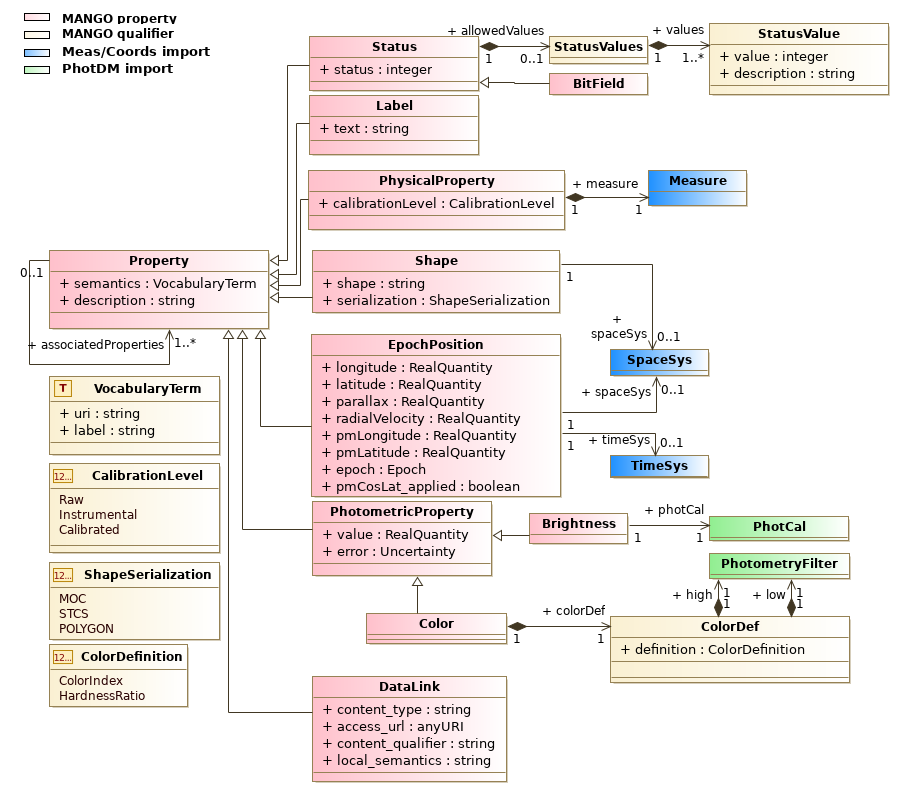
\includegraphics[width=1.0\textwidth]{../model/property.png}
        \caption{MANGO Properties}
        \label{fig:property}
      \end{figure}

\subsubsection{Supported Properties}

\begin{table}[h!]
\small
\begin{center}
\begin{tabular}{|| p{3.5cm} | p{3.5cm} |  p{3.5cm} ||} 
 \hline\hline
 \textbf{Property} & \textbf{Purpose} & \textbf{Example} \\ 
  \hline\hline
 \texttt{Status} & Attach explicit labels to flag values & Chandra detection flag  \\ 
 \hline
 \texttt{Label} & Attach semantics to text label & Object name \\
 \hline
 \texttt{PhysicalProperty} & Hook for \texttt{Measure} classes & Model a columns as a time stamp \\
 \hline
 \texttt{Shape} & String serialization of shapes & Sky Coverage of a dust cloud \\
 \hline
 \texttt{EpochPosition} & Grouping of position with velocity and time & Parameters to solve the epoch propagation case\\  
 \hline
 \texttt{PhotometricProperty} & Flux or Magnitude & many \\ 
 \hline
 \texttt{Color} & Hardness ratio or magnitude ratio & many  \\ [1ex] 
 \hline
 \texttt{DataLink} & Flat representation of DataLink responses & Links to associated data given as column values\\ [1ex] 
 \hline
\end{tabular}
\caption{Properties supported by MANGO.}
\label{table:properties}
\end{center}
 \end{table}
This initial release supports a limited list of properties, listed in table \ref{table:properties}, that address the most common use cases.



All of these components are described in alphabetical order in the next section.

\subsubsection{Property Identification}
Since the set of properties associated with a particular instance is not defined by the model,
MANGO cannot define a specific role for each property. However, the model provides different ways
for the client to understand the actual nature of each property:

\begin{itemize}[noitemsep,topsep=0pt,parsep=0pt,partopsep=0pt]
    \item \textbf{Class type}: often the scientific meaning of the quantity.
    \item \textbf{Semantics}: the semantic tag specifies the exact role of the property by
          referring to a standard vocabulary. The semantic tag can relate to the property itself
          or to the set formed by the property and its associated properties.
          For example, a signal amplitude associated with a time and position can be tagged
          as a photon event.
    \item \textbf{Description}: free text description.
    \item \textbf{Literal attributes} : some property classes embed qualifiers telling 
          how the quantity must be interpreted (e.g. colour vs hardness ratio)
\end{itemize}


\subsubsection{MANGO and MIVOT: Structuring Tabular Data}

MANGO is primarily used to organise tabular data provided by TAP services \citep{2019ivoa.spec.0927D} 
other DAL nodes (one of the reference implementation is based on a Vizier SCS).
To achieve this, table rows must be linked to the model using MIVOT annotations.
We propose two strategies for establishing this mapping:
\begin{itemize}[noitemsep,topsep=0pt,parsep=0pt,partopsep=0pt]
    \item Single Object per Row: Each table row is treated as a single object,
          with its properties grouped within a container or dock.
    \item Scattered Independent Quantities: Each table row is considered as a collection of independent quantities.
\end{itemize}

\hfill \break

MIVOT annotations support both approaches:

\begin{itemize}[noitemsep,topsep=0pt,parsep=0pt,partopsep=0pt]
    \item MANGO as a Global View: This configuration enables full utilisation of the 
          model's features. Properties can be interconnected, data rows can be identified
          and treated as individual entities (MANGO objects) that can be linked together to describe,
          for example, sources with their detections or orbiting systems.
          This approach allows for serialisation formats like XML or JSON, which often require
          a unique root.
          However, the annotation process might be slightly more complex due to additional class levels.
    \item MANGO as a Sparse Parameter View: In this simpler approach, the data mapping is a
          flat set of independent objects. Clients can iterate through these objects and process
          the entities of interest individually.
          It's important to note that such a client could also handle data mapped to the full MANGO schema.
          The annotation process might be less complex on the server side.
\end{itemize}

This document does not favour one approach over the other.
The decision ultimately rests with the data providers.
However, both options are based on the full-featured MANGO model.

%
% -------------------------------------------
% Items to substitute into the ivoatex document template.
%
%\ivoagroup{Data Model Working Group}

%\title{Mango}


%\author{Laurent Michel}
    
%\author{Fran??ois Bonnarel}
    
%\author{Gilles Landais}
    
%\author{Mireille Louys}
    
%\author{Marco Molinaro}
    
%\author{Jesue Salgado}
    
%\previousversion{0.0}
      
% -------------------------------------------

\pagebreak
\section{Model: mango }
  
  % INSERT FIGURE HERE
  %\begin{figure}[h]
  %\begin{center}
  %  \includegraphics[width=\textwidth]{????.png}
  %  \caption{???}\label{fig:????}
  %\end{center}
  %\end{figure}

  The purpose of MANGO, which stands for MO-del for AN-notating G-eneric O-objects, is to add an upper level of description to the tabular data of query responses. It allows metadata to be extended, complex quantities to be reconstructed from column values, and properties to be linked. It also allows to specify the origin af the data.

  \subsection{AssociatedMangoObject}
  \label{sect:AssociatedMangoObject}
    This class gives the role of a link associating 2 \texttt{MangoObject} together.

    \subsubsection{AssociatedMangoObject.semantics}
      \textbf{vodml-id: AssociatedMangoObject.semantics} \newline
      \textbf{type: \hyperref[sect:VocabularyTerm]{mango:VocabularyTerm}} \newline
      \textbf{multiplicity: 1} \newline
      Semantic concept giving the nature of the data association.

    \subsubsection{AssociatedMangoObject.description}
      \textbf{vodml-id: AssociatedMangoObject.description} \newline
      \textbf{type: \hyperref[sect:ivoa]{ivoa:string}} \newline
      \textbf{multiplicity: 1} \newline
      Free text description of the data association

    \subsubsection{AssociatedMangoObject.mangoObject}
      \textbf{vodml-id: AssociatedMangoObject.mangoObject} \newline
      \textbf{type: \hyperref[sect:MangoObject]{mango:MangoObject}} \newline
      \textbf{multiplicity: 1} \newline
      Reference to the associated \texttt{MangoObject}.

  \subsection{BitField}
  \label{sect:BitField}
    Property for which each possible value is represented by a bit, so that multiple states can be contained in the same integer value. The possible values are defined in the associated \texttt{StatusValues}, which must correspond to a bit pattern (each value must be a power of 2). This constraint is not enforced by the model.

  \subsection{Brightness}
  \label{sect:Brightness}
    Observed brightness of the \texttt{MangoObject}. The distinction between fluxes and magnitudes is made by the unit. This property should refer to a photometric calibration as defined by the \texttt{Phot} data model (1.1).

    \subsubsection{Brightness.photCal}
      \textbf{vodml-id: Brightness.photCal} \newline
      \textbf{type: Phot:PhotCal} \newline
      \textbf{multiplicity: 1} \newline
      Photometric calibration that applies to the photometric property. It must be an instance of \texttt{photdm:PhotCal}.

  \subsection{Color}
  \label{sect:Color}
    Property that describes a color of the \texttt{MangoObject}. The color is not an intrinsic property of the MANGO object, but a value relative to two filters or energy bands.

    \subsubsection{Color.colorDef}
      \textbf{vodml-id: Color.colorDef} \newline
      \textbf{type: \hyperref[sect:ColorDef]{mango:ColorDef}} \newline
      \textbf{multiplicity: 1} \newline
      Reference to the physical definition of the color (can be either a difference of magnitudes or a hardness ratio).

  \subsection{ColorDef}
  \label{sect:ColorDef}
    Physical color definition giving the way a color is calculated (magnitude difference or hardness ratio) and the filters on which the color is based. In case of hardness ratio, the energy bands might be modeled as instances of \texttt{Phot:PhotometryFilter} with a square transfert function.

    \subsubsection{ColorDef.definition}
      \textbf{vodml-id: ColorDef.definition} \newline
      \textbf{type: \hyperref[sect:ColorDefinition]{mango:ColorDefinition}} \newline
      \textbf{multiplicity: 1} \newline
      Attribute giving the way the color is calculated (magnitude difference or hardness ratio).

    \subsubsection{ColorDef.high}
      \textbf{vodml-id: ColorDef.high} \newline
      \textbf{type: Phot:PhotometryFilter} \newline
      \textbf{multiplicity: 1} \newline
      Reference to the \texttt{Phot:PhotometryFilter} \citep{2022ivoa.spec.1101S} corresponding the higher band of the color.

    \subsubsection{ColorDef.low}
      \textbf{vodml-id: ColorDef.low} \newline
      \textbf{type: Phot:PhotometryFilter} \newline
      \textbf{multiplicity: 1} \newline
      Reference to the \texttt{Phot:PhotometryFilter} corresponding the lower band for that color.

  \subsection{DataLink}
  \label{sect:DataLink}
    This property describes static links pointing to some external data. This allows services that do not implement DataLink services to expose linked data as flattened DataLink (1.1) responses.

    \subsubsection{DataLink.content\_type}
      \textbf{vodml-id: DataLink.content\_type} \newline
      \textbf{type: \hyperref[sect:ivoa]{ivoa:string}} \newline
      \textbf{multiplicity: 1} \newline
      mime type of the content the link returns (see DataLink 1.1)

    \subsubsection{DataLink.access\_url}
      \textbf{vodml-id: DataLink.access\_url} \newline
      \textbf{type: \hyperref[sect:ivoa]{ivoa:anyURI}} \newline
      \textbf{multiplicity: 1} \newline
      contains an URL for downloading a single resource. There is no restriction on the type of resource accessed by the links.

    \subsubsection{DataLink.content\_qualifier}
      \textbf{vodml-id: DataLink.content\_qualifier} \newline
      \textbf{type: \hyperref[sect:ivoa]{ivoa:string}} \newline
      \textbf{multiplicity: 1} \newline
      Gives the nature of the thing or service that is returned by the link. The value is always interpreted as a URI. If the access\_url references a data product, the content\_qualifier field should define its product type . In this case the content qualifier value always starts with a hash completing the \url{http://www.ivoa.net/rdf/datalink/product-type} base URI. For \texttt{MangoObject} not linking to data products, content\_qualifier’s interpretation will be different, and the default vocabulary will be inappropriate. Full concept URIs will have to be used in this case. (DataLink 1.1)

    \subsubsection{DataLink.local\_semantics}
      \textbf{vodml-id: DataLink.local\_semantics} \newline
      \textbf{type: \hyperref[sect:ivoa]{ivoa:string}} \newline
      \textbf{multiplicity: 1} \newline
      Allows for identification of corresponding rows for different IDs in the same DataLink service where the combination of semantics, content\_type and content\_qualifier is not sufficient to identify them (see DataLink 1.1).

  \subsection{EpochPosition}

      \begin{figure}[h]
        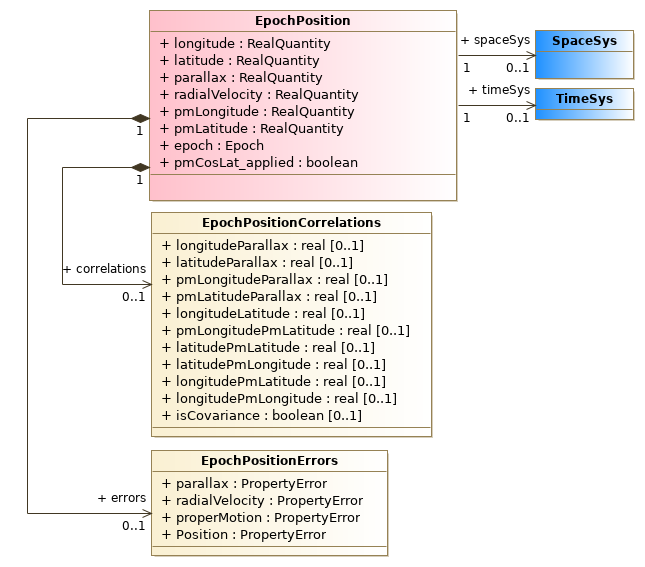
\includegraphics[width=1.0\textwidth]{../model/EpochPosition.png}
        \caption{Class EpochPosition}
        \label{fig:EpochPosition}
      \end{figure}

    
  \label{sect:EpochPosition}
    This class (fig \ref{fig:EpochPosition}) is a view of \texttt{Astronomical Coordinates and Coordinate Systems} \citep{2022ivoa.specQ1004R} components that have been put together to form a consistent description of the position of an object moving over time. It consists of a celestial position, a proper motion, a radial velocity and a parallax. All components share the same coordinate systems for both time and space coordinates. \begin{itemize} \item Both position and proper motion reuse \texttt{coords:LonLatPoint} elements. \item The space coordinate system is imported from \texttt{coords:spaceSys}. \item The time coordinate system is imported from \texttt{coords:timeSys}. \end{itemize} The \texttt{EpochPosition} error is modeled by specific classes supporting covariance and/or correlation between components. All individual components have their own units which must be consistent to each others. This consistency is not enforced by the model. Possible correlations between \texttt{EpochPosition} parameters are handle by the \texttt{EpochPositionCorrelation} class.

    \subsubsection{EpochPosition.longitude}
      \textbf{vodml-id: EpochPosition.longitude} \newline
      \textbf{type: \hyperref[sect:ivoa]{ivoa:RealQuantity}} \newline
      \textbf{multiplicity: 1} \newline
      The longitude of the Point, as a Quantity with angular units (see \texttt{coords:LonLatPoint.lon}.

    \subsubsection{EpochPosition.latitude}
      \textbf{vodml-id: EpochPosition.latitude} \newline
      \textbf{type: \hyperref[sect:ivoa]{ivoa:RealQuantity}} \newline
      \textbf{multiplicity: 1} \newline
      The latitude of the Point, as a Quantity with angular units (see \texttt{coords:LonLatPoint.lat}.

    \subsubsection{EpochPosition.parallax}
      \textbf{vodml-id: EpochPosition.parallax} \newline
      \textbf{type: \hyperref[sect:ivoa]{ivoa:RealQuantity}} \newline
      \textbf{multiplicity: 1} \newline
      The measured parallax in the coordinate system of the \texttt{EpochPosition} instance.

    \subsubsection{EpochPosition.radialVelocity}
      \textbf{vodml-id: EpochPosition.radialVelocity} \newline
      \textbf{type: \hyperref[sect:ivoa]{ivoa:RealQuantity}} \newline
      \textbf{multiplicity: 1} \newline
      The measured Velocity along of the radius axis (see \texttt{meas:Velocity.coord} in \cite{2022ivoa.spec.1004R}).

    \subsubsection{EpochPosition.pmLongitude}
      \textbf{vodml-id: EpochPosition.pmLongitude} \newline
      \textbf{type: \hyperref[sect:ivoa]{ivoa:RealQuantity}} \newline
      \textbf{multiplicity: 1} \newline
      Velocity along the longitude axis in angular distance per unit time (see \texttt{meas:ProperMotion.coord}). The current version of the model only allows a representation in the Polar coordinate space.

    \subsubsection{EpochPosition.pmLatitude}
      \textbf{vodml-id: EpochPosition.pmLatitude} \newline
      \textbf{type: \hyperref[sect:ivoa]{ivoa:RealQuantity}} \newline
      \textbf{multiplicity: 1} \newline
      Velocity along the latitude axis in angular distance per unit time (see \texttt{meas:ProperMotion.coord}). The current version of the model only allows a representation in the Polar coordinate space.

    \subsubsection{EpochPosition.epoch}
      \textbf{vodml-id: EpochPosition.epoch} \newline
      \textbf{type: coords:Epoch} \newline
      \textbf{multiplicity: 1} \newline
      Position epoch expressed within the common time system (see \texttt{coords:epoch})

    \subsubsection{EpochPosition.pmCosLat\_applied}
      \textbf{vodml-id: EpochPosition.pmCosLat\_applied} \newline
      \textbf{type: \hyperref[sect:ivoa]{ivoa:boolean}} \newline
      \textbf{multiplicity: 1} \newline
      It is common, though not universal, practice to quote longitudinal proper motion pre-multiplied by cos(latitude) so that the magnitude of the quantity is not affected by its longitudinal position. We do not constrain the value to one form or the other in this model. Instead, this flag enables providers to convey whether or not the factor has been applied (see \texttt{meas:ProperMotion.cosLat\_applied})

    \subsubsection{EpochPosition.errors}
      \textbf{vodml-id: EpochPosition.errors} \newline
      \textbf{type: \hyperref[sect:EpochPositionErrors]{mango:EpochPositionErrors}} \newline
      \textbf{multiplicity: 0..1} \newline
      Reference to the combined errors of the \texttt{EpochPosition} components.

    \subsubsection{EpochPosition.correlations}
      \textbf{vodml-id: EpochPosition.correlations} \newline
      \textbf{type: \hyperref[sect:EpochPositionCorrelations]{mango:EpochPositionCorrelations}} \newline
      \textbf{multiplicity: 0..1} \newline
      Reference to the correlations between the \texttt{EpochPosition} components.

    \subsubsection{EpochPosition.spaceSys}
      \textbf{vodml-id: EpochPosition.spaceSys} \newline
      \textbf{type: coords:SpaceSys} \newline
      \textbf{multiplicity: 0..1} \newline
      System that applies the space coordinates.

    \subsubsection{EpochPosition.timeSys}
      \textbf{vodml-id: EpochPosition.timeSys} \newline
      \textbf{type: coords:TimeSys} \newline
      \textbf{multiplicity: 0..1} \newline
      System that applies the time coordinates (the epoch).

  \subsection{EpochPositionCorrelations}
  \label{sect:EpochPositionCorrelations}
    Class holder for the correlation coefficients between the \texttt{EpochPosition} components.

    \subsubsection{EpochPositionCorrelations.longitudeParallax}
      \textbf{vodml-id: EpochPositionCorrelations.longitudeParallax} \newline
      \textbf{type: \hyperref[sect:ivoa]{ivoa:real}} \newline
      \textbf{multiplicity: 0..1} \newline
      Correlation (or covariance) coefficient between the position longitude and the parallax

    \subsubsection{EpochPositionCorrelations.latitudeParallax}
      \textbf{vodml-id: EpochPositionCorrelations.latitudeParallax} \newline
      \textbf{type: \hyperref[sect:ivoa]{ivoa:real}} \newline
      \textbf{multiplicity: 0..1} \newline
      Correlation (or covariance) coefficient between the position latitude and the parallax

    \subsubsection{EpochPositionCorrelations.pmLongitudeParallax}
      \textbf{vodml-id: EpochPositionCorrelations.pmLongitudeParallax} \newline
      \textbf{type: \hyperref[sect:ivoa]{ivoa:real}} \newline
      \textbf{multiplicity: 0..1} \newline
      Correlation (or covariance) coefficient between the proper motion longitude and the parallax

    \subsubsection{EpochPositionCorrelations.pmLatitudeParallax}
      \textbf{vodml-id: EpochPositionCorrelations.pmLatitudeParallax} \newline
      \textbf{type: \hyperref[sect:ivoa]{ivoa:real}} \newline
      \textbf{multiplicity: 0..1} \newline
      Correlation (or covariance) coefficient between the proper motion latitude and the parallax

    \subsubsection{EpochPositionCorrelations.longitudeLatitude}
      \textbf{vodml-id: EpochPositionCorrelations.longitudeLatitude} \newline
      \textbf{type: \hyperref[sect:ivoa]{ivoa:real}} \newline
      \textbf{multiplicity: 0..1} \newline
      Correlation (or covariance) coefficient between the position longitude and the position latitude

    \subsubsection{EpochPositionCorrelations.pmLongitudePmLatitude}
      \textbf{vodml-id: EpochPositionCorrelations.pmLongitudePmLatitude} \newline
      \textbf{type: \hyperref[sect:ivoa]{ivoa:real}} \newline
      \textbf{multiplicity: 0..1} \newline
      Correlation (or covariance) coefficient between the proper motion longitude and the proper motion latitude

    \subsubsection{EpochPositionCorrelations.latitudePmLatitude}
      \textbf{vodml-id: EpochPositionCorrelations.latitudePmLatitude} \newline
      \textbf{type: \hyperref[sect:ivoa]{ivoa:real}} \newline
      \textbf{multiplicity: 0..1} \newline
      Correlation (or covariance) coefficient between the position latitude and the proper motion latitude

    \subsubsection{EpochPositionCorrelations.latitudePmLongitude}
      \textbf{vodml-id: EpochPositionCorrelations.latitudePmLongitude} \newline
      \textbf{type: \hyperref[sect:ivoa]{ivoa:real}} \newline
      \textbf{multiplicity: 0..1} \newline
      Correlation (or covariance) coefficient between the position latitude and the proper motion longitude

    \subsubsection{EpochPositionCorrelations.longitudePmLatitude}
      \textbf{vodml-id: EpochPositionCorrelations.longitudePmLatitude} \newline
      \textbf{type: \hyperref[sect:ivoa]{ivoa:real}} \newline
      \textbf{multiplicity: 0..1} \newline
      Correlation (or covariance) coefficient between the position longitude and the proper motion latitude

    \subsubsection{EpochPositionCorrelations.longitudePmLongitude}
      \textbf{vodml-id: EpochPositionCorrelations.longitudePmLongitude} \newline
      \textbf{type: \hyperref[sect:ivoa]{ivoa:real}} \newline
      \textbf{multiplicity: 0..1} \newline
      Correlation (or covariance) coefficient between the position longitude and the proper motion longitude

    \subsubsection{EpochPositionCorrelations.isCovariance}
      \textbf{vodml-id: EpochPositionCorrelations.isCovariance} \newline
      \textbf{type: \hyperref[sect:ivoa]{ivoa:boolean}} \newline
      \textbf{multiplicity: 0..1} \newline
      Boolean telling whether the correlations must be interpreted as covariance or as correlation coefficients.

  \subsection{EpochPositionErrors}
  \label{sect:EpochPositionErrors}
    Class holder for the errors of the EpochPosition attributes

    \subsubsection{EpochPositionErrors.parallax}
      \textbf{vodml-id: EpochPositionErrors.parallax} \newline
      \textbf{type: \hyperref[sect:error.PropertyError]{mango:error.PropertyError}} \newline
      \textbf{multiplicity: 1} \newline
      Parallax error. This error is meant to be symmetrical in the current model version.

    \subsubsection{EpochPositionErrors.radialVelocity}
      \textbf{vodml-id: EpochPositionErrors.radialVelocity} \newline
      \textbf{type: \hyperref[sect:error.PropertyError]{mango:error.PropertyError}} \newline
      \textbf{multiplicity: 1} \newline
      Error in the radial velocity. This error is meant to be symmetrical in the current model version.

    \subsubsection{EpochPositionErrors.properMotion}
      \textbf{vodml-id: EpochPositionErrors.properMotion} \newline
      \textbf{type: \hyperref[sect:error.PropertyError]{mango:error.PropertyError}} \newline
      \textbf{multiplicity: 1} \newline
      Position error; can be an ellipse, a correlation matrix or a covariance matrix.

    \subsubsection{EpochPositionErrors.Position}
      \textbf{vodml-id: EpochPositionErrors.Position} \newline
      \textbf{type: \hyperref[sect:error.PropertyError]{mango:error.PropertyError}} \newline
      \textbf{multiplicity: 1} \newline
      Position error; can be an ellipse, a correlation matrix or a covariance matrix.

  \subsection{Label}
  \label{sect:Label}
    Free text label seen as a MANGO object property.

    \subsubsection{Label.text}
      \textbf{vodml-id: Label.text} \newline
      \textbf{type: \hyperref[sect:ivoa]{ivoa:string}} \newline
      \textbf{multiplicity: 1} \newline
      Text of label property of the MANGO object.

  \subsection{MangoObject}
  \label{sect:MangoObject}
    Central model class: applied to a data table, each row can be modelled as a \texttt{MangoObject} instance. Each \texttt{MangoObject} hosts a collection of physical or calculated parameters, a description of the data origin and an identifier.

    \subsubsection{MangoObject.identifier}
      \textbf{vodml-id: MangoObject.identifier} \newline
      \textbf{type: \hyperref[sect:ivoa]{ivoa:string}} \newline
      \textbf{multiplicity: 1} \newline
      Unique identifier of the \texttt{MangoObject}. The uniqueness of that identifier is not managed by the model. The format is free.

    \subsubsection{MangoObject.propertyDock}
      \textbf{vodml-id: MangoObject.propertyDock} \newline
      \textbf{type: \hyperref[sect:Property]{mango:Property}} \newline
      \textbf{multiplicity: 0..*} \newline
      Reference to the open-ended collection of the \texttt{MangoObject} properties (physical or calculated).

    \subsubsection{MangoObject.dataOrigin}
      \textbf{vodml-id: MangoObject.dataOrigin} \newline
      \textbf{type: \hyperref[sect:dataorigin.DataOrigin]{mango:dataorigin.DataOrigin}} \newline
      \textbf{multiplicity: 0..1} \newline
      Reference to the description of the origin of the \texttt{MangoObject}.

    \subsubsection{MangoObject.associatedMangoObjects}
      \textbf{vodml-id: MangoObject.associatedMangoObjects} \newline
      \textbf{type: \hyperref[sect:AssociatedMangoObject]{mango:AssociatedMangoObject}} \newline
      \textbf{multiplicity: 0..*} \newline
      Abstract reference to a particular dataset associated to the MANGO entity. This class is used to specify the type of the associated dataset as well as its role.

  \subsection{PhotometricProperty}
  \label{sect:PhotometricProperty}
    Super class for all photometric properties of the \texttt{MangoObject}.

    \subsubsection{PhotometricProperty.value}
      \textbf{vodml-id: PhotometricProperty.value} \newline
      \textbf{type: \hyperref[sect:ivoa]{ivoa:RealQuantity}} \newline
      \textbf{multiplicity: 1} \newline
      Value of the photometric property associated with a photometric calibration as defined by the \texttt{PhotDM} model.

    \subsubsection{PhotometricProperty.error}
      \textbf{vodml-id: PhotometricProperty.error} \newline
      \textbf{type: meas:Uncertainty} \newline
      \textbf{multiplicity: 1} \newline
      Error on the \texttt{PhotometricProperty}, imported from \texttt{meas:Uncertainty}.

  \subsection{PhysicalProperty}
  \label{sect:PhysicalProperty}
    Place holder for any quantity that can be hold by measure classes as defined in the \texttt{Astronomical Measurements Model}.

    \subsubsection{PhysicalProperty.calibrationLevel}
      \textbf{vodml-id: PhysicalProperty.calibrationLevel} \newline
      \textbf{type: \hyperref[sect:CalibrationLevel]{mango:CalibrationLevel}} \newline
      \textbf{multiplicity: 1} \newline
      Calibration level of the property as defined in ObsCore \citep{2011ivoa.spec.1028T}.

    \subsubsection{PhysicalProperty.measure}
      \textbf{vodml-id: PhysicalProperty.measure} \newline
      \textbf{type: meas:Measure} \newline
      \textbf{multiplicity: 1} \newline
      Instance of \texttt{Astronomical Measurements Model} that holds the Property value(s).

  \subsection{Property}
  \label{sect:Property}
    Class holder for a particular property, either physical or calculated, of the MANGO object. This class specifies both type and role of the property, and hosts the property instance itself.

    \noindent \textbf{constraint} \newline
    \indent    \textbf{detail: Property.One association at the time
 }\newline


    \subsubsection{Property.semantics}
      \textbf{vodml-id: Property.semantics} \newline
      \textbf{type: \hyperref[sect:VocabularyTerm]{mango:VocabularyTerm}} \newline
      \textbf{multiplicity: 1} \newline
      Reference to a semantic concept giving the nature of the property or of the set made of the property and its associated properties. The semantics field contains a URI for a concept that describes the meaning of the property. This attribute is intended to be machine-readable and to assist automated link selection, presentation, and usage. The value is always interpreted as a URI; relative URIs (Berners-Lee and Fielding et al., 2005) are completed using the base URI of the core DataLink vocabulary, http://www.ivoa.net/rdf/datalink/core. Terms from this vocabulary must always be written as relative URIs. This means that for concepts from the core vocabulary, the value in the semantics fieldz always starts with a hash. (datalink1.1). The semantic concept apply to a single property or to the set made of the property and its associated properties (e.g. position and flag).

    \subsubsection{Property.description}
      \textbf{vodml-id: Property.description} \newline
      \textbf{type: \hyperref[sect:ivoa]{ivoa:string}} \newline
      \textbf{multiplicity: 1} \newline
      Free text description of the property or of the set made of the property and its associated properties.

    \subsubsection{Property.associatedProperties}
      \textbf{vodml-id: Property.associatedProperties} \newline
      \textbf{type: \hyperref[sect:Property]{mango:Property}} \newline
      \textbf{multiplicity: 1..*} \newline
      Open-ended collection of MANGO properties associated with the \texttt{MangoObject}. These relationships are typically used to associate physical properties with time stamps and/or quality factors.

  \subsection{Shape}
  \label{sect:Shape}
    Description of the spatial extension of the MANGO object (for e.g. dust clouds)

    \subsubsection{Shape.shape}
      \textbf{vodml-id: Shape.shape} \newline
      \textbf{type: \hyperref[sect:ivoa]{ivoa:string}} \newline
      \textbf{multiplicity: 1} \newline
      String serialization of the spatial extension of the \texttt{MangoObject}

    \subsubsection{Shape.serialization}
      \textbf{vodml-id: Shape.serialization} \newline
      \textbf{type: \hyperref[sect:ShapeSerialization]{mango:ShapeSerialization}} \newline
      \textbf{multiplicity: 1} \newline
      Serialization mode of the spatial extension of the MANGO entity

    \subsubsection{Shape.spaceSys}
      \textbf{vodml-id: Shape.spaceSys} \newline
      \textbf{type: coords:SpaceSys} \newline
      \textbf{multiplicity: 0..1} \newline
      Coordinate system that applies for the shape

  \subsection{Status}
  \label{sect:Status}
    Property representing a status defined by a integer number that can only take on a defined number of values, each with its own description. Boolean status can be represented by \texttt{StatusValues} with 2 values e.g. 0 for False and 1 for True.

    \subsubsection{Status.status}
      \textbf{vodml-id: Status.status} \newline
      \textbf{type: \hyperref[sect:ivoa]{ivoa:integer}} \newline
      \textbf{multiplicity: 1} \newline
      Actual value of the status

    \subsubsection{Status.allowedValues}
      \textbf{vodml-id: Status.allowedValues} \newline
      \textbf{type: \hyperref[sect:StatusValues]{mango:StatusValues}} \newline
      \textbf{multiplicity: 0..1} \newline
      List of the allowed values for the status. Each value has its own free text description.

  \subsection{StatusValue}
  \label{sect:StatusValue}
    Value allowed for a status; contain the value with a free text description.

    \subsubsection{StatusValue.value}
      \textbf{vodml-id: StatusValue.value} \newline
      \textbf{type: \hyperref[sect:ivoa]{ivoa:integer}} \newline
      \textbf{multiplicity: 1} \newline
      Allowed value for a \texttt{Status}

    \subsubsection{StatusValue.description}
      \textbf{vodml-id: StatusValue.description} \newline
      \textbf{type: \hyperref[sect:ivoa]{ivoa:string}} \newline
      \textbf{multiplicity: 1} \newline
      Free text description of the allowed value for a \texttt{Status}

  \subsection{StatusValues}
  \label{sect:StatusValues}
    Class holder for the list of the allowed values for the status.

    \subsubsection{StatusValues.values}
      \textbf{vodml-id: StatusValues.values} \newline
      \textbf{type: \hyperref[sect:StatusValue]{mango:StatusValue}} \newline
      \textbf{multiplicity: 1..*} \newline
      List of the allowed values for the status; each value has its own textual description.

  \subsection{VocabularyTerm}
  \label{sect:VocabularyTerm}
    Class holder for a term of a standardized vocabulary that applies to a property.

    \subsubsection{VocabularyTerm.uri}
      \textbf{vodml-id: VocabularyTerm.uri} \newline
      \textbf{type: \hyperref[sect:ivoa]{ivoa:string}} \newline
      \textbf{multiplicity: 1} \newline
      URI the vocabulary term

    \subsubsection{VocabularyTerm.label}
      \textbf{vodml-id: VocabularyTerm.label} \newline
      \textbf{type: \hyperref[sect:ivoa]{ivoa:string}} \newline
      \textbf{multiplicity: 1} \newline
      Label attached to the vocabulary term. This is necessary because the URI may not contain any explicit label. This was the case for the IUA vocabulary until the Registry WG introduced rewriting rules that fix the issue.

  \subsection{ShapeFrame}
  \label{sect:ShapeFrame}

  Possible schemes to encode a shape in a string

  \noindent \underline{Enumeration Literals}
  \vspace{-\parsep}
  \small
  \begin{itemize}
  
    \item[\textbf{STC\_S}]: \textbf{vodml-id:} ShapeFrame.STC\_S \newline
          \textbf{description:} MOC serialization
    \item[\textbf{MOC}]: \textbf{vodml-id:} ShapeFrame.MOC \newline
          \textbf{description:} MOC serialization
  \end{itemize}
  \normalsize


  \subsection{ShapeSerialization}
  \label{sect:ShapeSerialization}

  Enumeration of the supported serialization modes for the shapes

  \noindent \underline{Enumeration Literals}
  \vspace{-\parsep}
  \small
  \begin{itemize}
  
    \item[\textbf{MOC}]: \textbf{vodml-id:} ShapeSerialization.MOC \newline
          \textbf{description:} Label indicating that the shape has been serialized as a S-MOC
    \item[\textbf{STCS}]: \textbf{vodml-id:} ShapeSerialization.STCS \newline
          \textbf{description:} Label indicating that the shape has been serialized as a STC-S \citep{2007ivoa.spec.1030R} string
    \item[\textbf{POLYGON}]: \textbf{vodml-id:} ShapeSerialization.POLYGON \newline
          \textbf{description:} Label indicating that the shape has been serialized as a polygon (cf xtypes)
  \end{itemize}
  \normalsize


  \subsection{CalibrationLevel}
  \label{sect:CalibrationLevel}

  Enumeration of different possible calibration status of the property as defined in Obscore

  \noindent \underline{Enumeration Literals}
  \vspace{-\parsep}
  \small
  \begin{itemize}
  
    \item[\textbf{Raw}]: \textbf{vodml-id:} CalibrationLevel.Raw \newline
          \textbf{description:} Raw instrumental data, in a proprietary or internal data provider defined format, that needs instrument specific tools to be handled (ObsCore)
    \item[\textbf{Instrumental}]: \textbf{vodml-id:} CalibrationLevel.Instrumental \newline
          \textbf{description:} Instrumental data in a standard format which could be manipulated with standard astronomical packages (ObsCore).
    \item[\textbf{Calibrated}]: \textbf{vodml-id:} CalibrationLevel.Calibrated \newline
          \textbf{description:} Science ready data with the instrument signature removed (ObsCore)
  \end{itemize}
  \normalsize


  \subsection{ColorDefinition}
  \label{sect:ColorDefinition}

  Enumeration of the different types of colors supported by the model.

  \noindent \underline{Enumeration Literals}
  \vspace{-\parsep}
  \small
  \begin{itemize}
  
    \item[\textbf{ColorIndex}]: \textbf{vodml-id:} ColorDefinition.ColorIndex \newline
          \textbf{description:} Difference of magnitudes: typically $M_B - M_v$
    \item[\textbf{HardnessRatio}]: \textbf{vodml-id:} ColorDefinition.HardnessRatio \newline
          \textbf{description:} Normalized ratio of fluxes: $(F_{EB2} - F_{EB1}) / (F_{EB2} + F_{EB1})$
  \end{itemize}
  \normalsize


\pagebreak
\section{Package: error }
  \begin{figure}[h]
    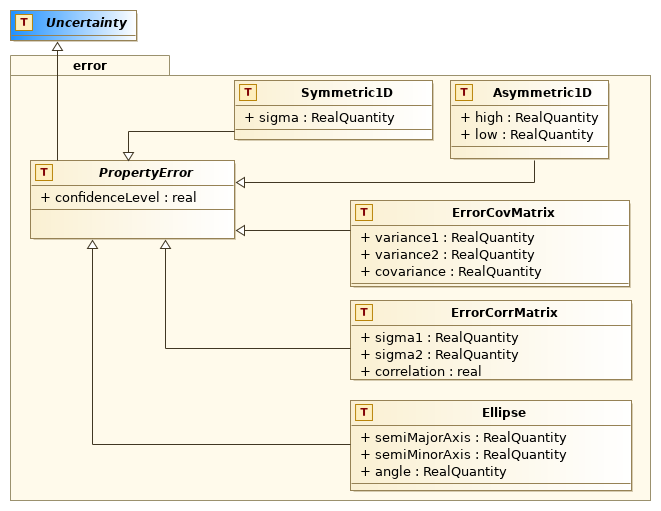
\includegraphics[width=1.0\textwidth]{../model/error.png}
    \caption{package error}
    \label{fig:error}
  \end{figure}



  % INSERT FIGURE HERE
  %\begin{figure}[h]
  %\begin{center}
  %  \includegraphics[width=\textwidth]{????.png}
  %  \caption{???}\label{fig:????}
  %\end{center}
  %\end{figure}

  The \texttt{error} package (fig \ref{fig:error}) groups the MANGO built-in error classes. All these classes are derived from \texttt{meas:Uncertainty} to make them reusable by \texttt{meas:Measure} instances. Mango errors all have an attribute that specifies the confidence level

  \subsection{Asymmetric1D}
  \label{sect:error.Asymmetric1D}
    Asymmetric error for 1D parameters

    \subsubsection{Asymmetric1D.high}
      \textbf{vodml-id: error.Asymmetric1D.high} \newline
      \textbf{type: \hyperref[sect:ivoa]{ivoa:RealQuantity}} \newline
      \textbf{multiplicity: 1} \newline
      High limit for the asymmetric error for 1D parameters

    \subsubsection{Asymmetric1D.low}
      \textbf{vodml-id: error.Asymmetric1D.low} \newline
      \textbf{type: \hyperref[sect:ivoa]{ivoa:RealQuantity}} \newline
      \textbf{multiplicity: 1} \newline
      Low limit for the asymmetric error for 1D parameters

  \subsection{Ellipse}
  \label{sect:error.Ellipse}
    Elliptic error for 2D parameters such as sky positions. Major axis and minor axis have their own units, which must be the same for both. This is not enforced by the model. The definition of the ellipse attribute is imported from \texttt{coords:Ellipse}.

    \subsubsection{Ellipse.semiMajorAxis}
      \textbf{vodml-id: error.Ellipse.semiMajorAxis} \newline
      \textbf{type: \hyperref[sect:ivoa]{ivoa:RealQuantity}} \newline
      \textbf{multiplicity: 1} \newline
      Half of the ellipse major axis

    \subsubsection{Ellipse.semiMinorAxis}
      \textbf{vodml-id: error.Ellipse.semiMinorAxis} \newline
      \textbf{type: \hyperref[sect:ivoa]{ivoa:RealQuantity}} \newline
      \textbf{multiplicity: 1} \newline
      Half of the ellipse minor axis

    \subsubsection{Ellipse.angle}
      \textbf{vodml-id: error.Ellipse.angle} \newline
      \textbf{type: \hyperref[sect:ivoa]{ivoa:RealQuantity}} \newline
      \textbf{multiplicity: 1} \newline
      Angle between the North Polar Cape (NCP) and the major axis. This angle must be positive taking into account that angles are positive from North to the East. The angle has its own unit.

  \subsection{ErrorCorrMatrix}
  \label{sect:error.ErrorCorrMatrix}
    Correlation matrix for the error of a 2D quantities. The correlation matrix is symmetrical.

    \subsubsection{ErrorCorrMatrix.sigma1}
      \textbf{vodml-id: error.ErrorCorrMatrix.sigma1} \newline
      \textbf{type: \hyperref[sect:ivoa]{ivoa:RealQuantity}} \newline
      \textbf{multiplicity: 1} \newline
      Error on the first dimension (right ascension in case of sky coordinates)

    \subsubsection{ErrorCorrMatrix.sigma2}
      \textbf{vodml-id: error.ErrorCorrMatrix.sigma2} \newline
      \textbf{type: \hyperref[sect:ivoa]{ivoa:RealQuantity}} \newline
      \textbf{multiplicity: 1} \newline
      Error on the second dimension (declination in case of sky coordinates)

    \subsubsection{ErrorCorrMatrix.correlation}
      \textbf{vodml-id: error.ErrorCorrMatrix.correlation} \newline
      \textbf{type: \hyperref[sect:ivoa]{ivoa:real}} \newline
      \textbf{multiplicity: 1} \newline
      Correlation coefficient between the 2 axis

  \subsection{ErrorCovMatrix}
  \label{sect:error.ErrorCovMatrix}
    Covariance matrix for the error of a 2D quantities. The covariance matrix is symmetrical.

    \subsubsection{ErrorCovMatrix.variance1}
      \textbf{vodml-id: error.ErrorCovMatrix.variance1} \newline
      \textbf{type: \hyperref[sect:ivoa]{ivoa:RealQuantity}} \newline
      \textbf{multiplicity: 1} \newline
      Variance of the first dimension (right ascension in case of sky coordinates)

    \subsubsection{ErrorCovMatrix.variance2}
      \textbf{vodml-id: error.ErrorCovMatrix.variance2} \newline
      \textbf{type: \hyperref[sect:ivoa]{ivoa:RealQuantity}} \newline
      \textbf{multiplicity: 1} \newline
      Variance of the second dimension (declination in case of sky coordinates)

    \subsubsection{ErrorCovMatrix.covariance}
      \textbf{vodml-id: error.ErrorCovMatrix.covariance} \newline
      \textbf{type: \hyperref[sect:ivoa]{ivoa:RealQuantity}} \newline
      \textbf{multiplicity: 1} \newline
      Covariance of the 2 axis

  \subsection{PropertyError (Abstract)}
  \label{sect:error.PropertyError}
    Root (abstract) class of the errors that can be attached to a MANGO property. The class inherits from \texttt{meas:uncertainty} in order to be usable in the context of properties based on \texttt{Measures} classes.

    \subsubsection{PropertyError.confidenceLevel}
      \textbf{vodml-id: error.PropertyError.confidenceLevel} \newline
      \textbf{type: \hyperref[sect:ivoa]{ivoa:real}} \newline
      \textbf{multiplicity: 1} \newline
      Confidence level of the error. The confidence level must be in $[0, 1]$ (not enforced by the VO-DML schema).

  \subsection{Symmetric1D}
  \label{sect:error.Symmetric1D}
    Symmetric error for 1D parameters

    \subsubsection{Symmetric1D.sigma}
      \textbf{vodml-id: error.Symmetric1D.sigma} \newline
      \textbf{type: \hyperref[sect:ivoa]{ivoa:RealQuantity}} \newline
      \textbf{multiplicity: 1} \newline
      Amplitude of the symmetric error on a one-dimensional parameter

\pagebreak
\section{Package: dataorigin }
  \begin{figure}[h]
    \includegraphics[width=1.0\textwidth]{../model/dataorigin.png}
    \caption{package dataorigin}
    \label{fig:dataorigin}
  \end{figure}



  % INSERT FIGURE HERE
  %\begin{figure}[h]
  %\begin{center}
  %  \includegraphics[width=\textwidth]{????.png}
  %  \caption{???}\label{fig:????}
  %\end{center}
  %\end{figure}

  Package grouping together all the components needed to model the origin of \texttt{MangoObject} (fig \ref{fig:dataorigin}).

  \subsection{Article}
  \label{sect:dataorigin.Article}
    Reference article for the MANGO entity

    \subsubsection{Article.editor}
      \textbf{vodml-id: dataorigin.Article.editor} \newline
      \textbf{type: \hyperref[sect:ivoa]{ivoa:string}} \newline
      \textbf{multiplicity: 1} \newline
      Name of the article editor

    \subsubsection{Article.code}
      \textbf{vodml-id: dataorigin.Article.code} \newline
      \textbf{type: \hyperref[sect:ivoa]{ivoa:string}} \newline
      \textbf{multiplicity: 1} \newline
      Bibcode or DOI of the reference article

  \subsection{DataOrigin}
  \label{sect:dataorigin.DataOrigin}
    Class representing the origin of the data following the DCP note

    \subsubsection{DataOrigin.citation}
      \textbf{vodml-id: dataorigin.DataOrigin.citation} \newline
      \textbf{type: \hyperref[sect:ivoa]{ivoa:string}} \newline
      \textbf{multiplicity: 1} \newline
      Dataset identifier that can be used for citation (e.g. DOI)

    \subsubsection{DataOrigin.reference\_url}
      \textbf{vodml-id: dataorigin.DataOrigin.reference\_url} \newline
      \textbf{type: \hyperref[sect:ivoa]{ivoa:string}} \newline
      \textbf{multiplicity: 1} \newline
      Dataset landing page

    \subsubsection{DataOrigin.resource\_version}
      \textbf{vodml-id: dataorigin.DataOrigin.resource\_version} \newline
      \textbf{type: \hyperref[sect:ivoa]{ivoa:string}} \newline
      \textbf{multiplicity: 1} \newline
      Dataset version

    \subsubsection{DataOrigin.creator}
      \textbf{vodml-id: dataorigin.DataOrigin.creator} \newline
      \textbf{type: \hyperref[sect:ivoa]{ivoa:string}} \newline
      \textbf{multiplicity: 1} \newline
      Person(s) mainly involved in the creation of the resource, generally the author

    \subsubsection{DataOrigin.cites}
      \textbf{vodml-id: dataorigin.DataOrigin.cites} \newline
      \textbf{type: \hyperref[sect:ivoa]{ivoa:string}} \newline
      \textbf{multiplicity: 1} \newline
      Identifier (IVOID, DOI or Bibcode) of a second Resource using relation of type \texttt{cites} (\url{https://www.ivoa.net/rdf/voresource/relationship\_type/})

    \subsubsection{DataOrigin.is\_derived\_from}
      \textbf{vodml-id: dataorigin.DataOrigin.is\_derived\_from} \newline
      \textbf{type: \hyperref[sect:ivoa]{ivoa:string}} \newline
      \textbf{multiplicity: 1} \newline
      Identifier (IVOID, DOI or Bibcode) of a second resource using relation of type \texttt{is\_derived\_from} (\url{https://www.ivoa.net/rdf/voresource/relationship\_type/})

    \subsubsection{DataOrigin.original\_date}
      \textbf{vodml-id: dataorigin.DataOrigin.original\_date} \newline
      \textbf{type: \hyperref[sect:ivoa]{ivoa:datetime}} \newline
      \textbf{multiplicity: 1} \newline
      Date of the original resource from which the MANGO object is derived

    \subsubsection{DataOrigin.query}
      \textbf{vodml-id: dataorigin.DataOrigin.query} \newline
      \textbf{type: \hyperref[sect:dataorigin.QueryOrigin]{mango:dataorigin.QueryOrigin}} \newline
      \textbf{multiplicity: 0..1} \newline
      Description of the request from which the data originates.

    \subsubsection{DataOrigin.rights}
      \textbf{vodml-id: dataorigin.DataOrigin.rights} \newline
      \textbf{type: \hyperref[sect:dataorigin.License]{mango:dataorigin.License}} \newline
      \textbf{multiplicity: 0..1} \newline
      Reference to the rights that apply to the data.

    \subsubsection{DataOrigin.article}
      \textbf{vodml-id: dataorigin.DataOrigin.article} \newline
      \textbf{type: \hyperref[sect:dataorigin.Article]{mango:dataorigin.Article}} \newline
      \textbf{multiplicity: 0..1} \newline
      Reference to the article from which the data originates.

  \subsection{License}
  \label{sect:dataorigin.License}
    Place holder for the license covering the MANGO instance

    \subsubsection{License.rights\_uri}
      \textbf{vodml-id: dataorigin.License.rights\_uri} \newline
      \textbf{type: \hyperref[sect:ivoa]{ivoa:string}} \newline
      \textbf{multiplicity: 1} \newline
      Licence URI. Following Registry practice, this should come from SPDX https://spdx.org/licenses/, though Creative Commons URLs https://creativecommons.org are also admitted.

    \subsubsection{License.rights}
      \textbf{vodml-id: dataorigin.License.rights} \newline
      \textbf{type: \hyperref[sect:ivoa]{ivoa:string}} \newline
      \textbf{multiplicity: 1} \newline
      License or Copyright text

  \subsection{QueryOrigin}
  \label{sect:dataorigin.QueryOrigin}
    Description of the query the MANGO instance results from.

    \subsubsection{QueryOrigin.ivoid}
      \textbf{vodml-id: dataorigin.QueryOrigin.ivoid} \newline
      \textbf{type: \hyperref[sect:ivoa]{ivoa:string}} \newline
      \textbf{multiplicity: 1} \newline
      IVOID of the underlying data collection

    \subsubsection{QueryOrigin.publisher}
      \textbf{vodml-id: dataorigin.QueryOrigin.publisher} \newline
      \textbf{type: \hyperref[sect:ivoa]{ivoa:string}} \newline
      \textbf{multiplicity: 1} \newline
      Data center that produced the MANGO instance

    \subsubsection{QueryOrigin.server\_software}
      \textbf{vodml-id: dataorigin.QueryOrigin.server\_software} \newline
      \textbf{type: \hyperref[sect:ivoa]{ivoa:string}} \newline
      \textbf{multiplicity: 1} \newline
      Version of the software the produced the MANGO object instance. It is encouraged to follow \url{https://ivoa.net/documents/Notes/softid/index.html}.

    \subsubsection{QueryOrigin.service\_protocol}
      \textbf{vodml-id: dataorigin.QueryOrigin.service\_protocol} \newline
      \textbf{type: \hyperref[sect:ivoa]{ivoa:string}} \newline
      \textbf{multiplicity: 1} \newline
      IVOID \citep{2007ivoa.spec.0314P} of the protocol through which the data was retrieved

    \subsubsection{QueryOrigin.request}
      \textbf{vodml-id: dataorigin.QueryOrigin.request} \newline
      \textbf{type: \hyperref[sect:ivoa]{ivoa:string}} \newline
      \textbf{multiplicity: 1} \newline
      Full request URL including a query string. For the simple protocols,put the url-encoded form of the query parameters. For TAP queries, use the /sync UWS \citep{2016ivoa.spec.1024H} URL. The format is free for others request types.

    \subsubsection{QueryOrigin.query}
      \textbf{vodml-id: dataorigin.QueryOrigin.query} \newline
      \textbf{type: \hyperref[sect:ivoa]{ivoa:string}} \newline
      \textbf{multiplicity: 1} \newline
      Input query in a formal langage such as ADQL.equest types \citep{2023ivoa.spec.1215M}

    \subsubsection{QueryOrigin.request\_date}
      \textbf{vodml-id: dataorigin.QueryOrigin.request\_date} \newline
      \textbf{type: \hyperref[sect:ivoa]{ivoa:datetime}} \newline
      \textbf{multiplicity: 1} \newline
      Query execution date

    \subsubsection{QueryOrigin.contact}
      \textbf{vodml-id: dataorigin.QueryOrigin.contact} \newline
      \textbf{type: \hyperref[sect:ivoa]{ivoa:string}} \newline
      \textbf{multiplicity: 1} \newline
      Email or URL to contact the publisher
\pagebreak

\section{Model: mango}

  \subsection{MangoObject}
    \label{sect:MangoObject}
    Central model class: applied to a data table, each row can be modelled as a \texttt{MangoObject} instance. Each \texttt{MangoObject} hosts a collection of physical or calculated parameters, a description of the data origin and an identifier.

    \subsubsection{MangoObject.identifier}
    \textbf{vodml-id: MangoObject.identifier} \newline
    \textbf{type: \hyperref[sect:ivoa]{ivoa:string}} \newline
    \textbf{multiplicity: 1} \newline
    Unique identifier of the \texttt{MangoObject}. The uniqueness of that identifier is not managed by the model. The format is free.

    \subsubsection{MangoObject.propertyDock}
    \textbf{vodml-id: MangoObject.propertyDock} \newline
    \textbf{type: \hyperref[sect:Property]{mango:Property}} \newline
    \textbf{multiplicity: 0..*} \newline
    Reference to the open-ended collection of the \texttt{MangoObject} properties (physical or calculated).

    \subsubsection{MangoObject.dataOrigin}
    \textbf{vodml-id: MangoObject.dataOrigin} \newline
    \textbf{type: \hyperref[sect:dataorigin.DataOrigin]{mango:dataorigin.DataOrigin}} \newline
    \textbf{multiplicity: 0..1} \newline
    Reference to the description of the origin of the \texttt{MangoObject}.

    \subsubsection{MangoObject.associatedMangoObjects}
    \textbf{vodml-id: MangoObject.associatedMangoObjects} \newline
    \textbf{type: \hyperref[sect:AssociatedMangoObject]{mango:AssociatedMangoObject}} \newline
    \textbf{multiplicity: 0..*} \newline
    Abstract reference to a particular dataset associated to the MANGO entity. This class is used to specify the type of the associated dataset as well as its role.

  \subsection{AssociatedMangoObject}
    \label{sect:AssociatedMangoObject}
    This class gives the role of a link associating 2 \texttt{MangoObject} together.

    \subsubsection{AssociatedMangoObject.semantics}
    \textbf{vodml-id: AssociatedMangoObject.semantics} \newline
    \textbf{type: \hyperref[sect:VocabularyTerm]{mango:VocabularyTerm}} \newline
    \textbf{multiplicity: 1} \newline
    Semantic concept giving the nature of the data association.

    \subsubsection{AssociatedMangoObject.description}
    \textbf{vodml-id: AssociatedMangoObject.description} \newline
    \textbf{type: \hyperref[sect:ivoa]{ivoa:string}} \newline
    \textbf{multiplicity: 1} \newline
    Free text description of the data association

    \subsubsection{AssociatedMangoObject.mangoObject}
    \textbf{vodml-id: AssociatedMangoObject.mangoObject} \newline
    \textbf{type: \hyperref[sect:MangoObject]{mango:MangoObject}} \newline
    \textbf{multiplicity: 1} \newline
    Reference to the associated \texttt{MangoObject}.

  \subsection{Property}
    \label{sect:Property}
    Class holder for a particular property, either physical or calculated, of the MANGO object. This class specifies both type and role of the property, and hosts the property instance itself.
    \noindent \textbf{constraint} \newline
    \indent    \textbf{detail: Property.One association at the time
    }\newline

    \subsubsection{Property.semantics}
    \textbf{vodml-id: Property.semantics} \newline
    \textbf{type: \hyperref[sect:VocabularyTerm]{mango:VocabularyTerm}} \newline
    \textbf{multiplicity: 1} \newline
    Reference to a semantic concept giving the nature of the property or of the set made of the property and its associated properties. The semantics field contains a URI for a concept that describes the meaning of the property. This attribute is intended to be machine-readable and to assist automated link selection, presentation, and usage. The value is always interpreted as a URI; relative URIs (Berners-Lee and Fielding et al., 2005) are completed using the base URI of the core DataLink vocabulary, http://www.ivoa.net/rdf/datalink/core. Terms from this vocabulary must always be written as relative URIs. This means that for concepts from the core vocabulary, the value in the semantics fieldz always starts with a hash. (datalink1.1). The semantic concept apply to a single property or to the set made of the property and its associated properties (e.g. position and flag).

    \subsubsection{Property.description}
    \textbf{vodml-id: Property.description} \newline
    \textbf{type: \hyperref[sect:ivoa]{ivoa:string}} \newline
    \textbf{multiplicity: 1} \newline
    Free text description of the property or of the set made of the property and its associated properties.

    \subsubsection{Property.associatedProperties}
    \textbf{vodml-id: Property.associatedProperties} \newline
    \textbf{type: \hyperref[sect:Property]{mango:Property}} \newline
    \textbf{multiplicity: 1..*} \newline
    Open-ended collection of MANGO properties associated with the \texttt{MangoObject}. These relationships are typically used to associate physical properties with time stamps and/or quality factors.

  \subsection{VocabularyTerm}
    \label{sect:VocabularyTerm}
    Class holder for a term of a standardized vocabulary that applies to a property.

    \subsubsection{VocabularyTerm.uri}
    \textbf{vodml-id: VocabularyTerm.uri} \newline
    \textbf{type: \hyperref[sect:ivoa]{ivoa:string}} \newline
    \textbf{multiplicity: 1} \newline
    URI the vocabulary term

    \subsubsection{VocabularyTerm.label}
    \textbf{vodml-id: VocabularyTerm.label} \newline
    \textbf{type: \hyperref[sect:ivoa]{ivoa:string}} \newline
    \textbf{multiplicity: 1} \newline
    Label attached to the vocabulary term. This is necessary because the URI may not contain any explicit label. This was the case for the IUA vocabulary until the Registry WG introduced rewriting rules that fix the issue.

\section{Epoch Position Properties}
This section collects all the classes that model the case of epoch propagation. 
In addition to the 6 sky position parameters, it also models their correlation and the errors.
  \subsection{EpochPosition}
    \begin{figure}[h]
    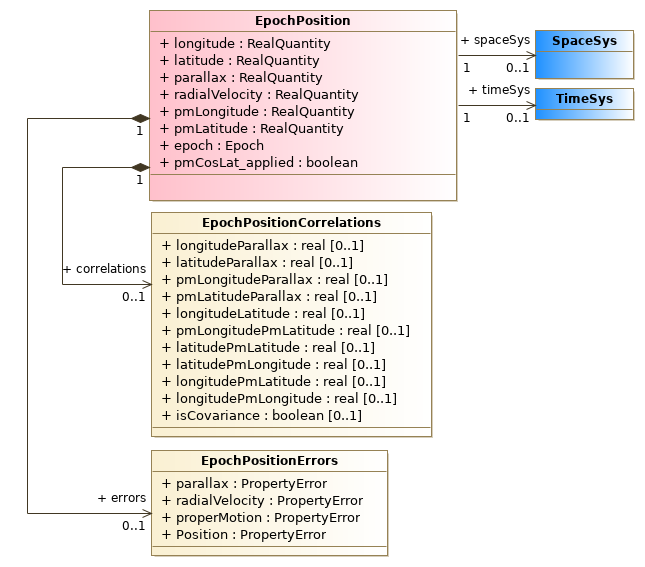
\includegraphics[width=1.0\textwidth]{../model/EpochPosition.png}
    \caption{Class EpochPosition}
    \label{fig:EpochPosition}
    \end{figure}
    \label{sect:EpochPosition}
    This class (fig \ref{fig:EpochPosition}) is a view of \texttt{Astronomical Coordinates and Coordinate Systems} \citep{2022ivoa.specQ1004R} components that have been put together to form a consistent description of the position of an object moving over time. It consists of a celestial position, a proper motion, a radial velocity and a parallax. All components share the same coordinate systems for both time and space coordinates. \begin{itemize} \item Both position and proper motion reuse \texttt{coords:LonLatPoint} elements. \item The space coordinate system is imported from \texttt{coords:spaceSys}. \item The time coordinate system is imported from \texttt{coords:timeSys}. \end{itemize} The \texttt{EpochPosition} error is modeled by specific classes supporting covariance and/or correlation between components. All individual components have their own units which must be consistent to each others. This consistency is not enforced by the model. Possible correlations between \texttt{EpochPosition} parameters are handle by the \texttt{EpochPositionCorrelation} class.

    \subsubsection{EpochPosition.longitude}
    \textbf{vodml-id: EpochPosition.longitude} \newline
    \textbf{type: \hyperref[sect:ivoa]{ivoa:RealQuantity}} \newline
    \textbf{multiplicity: 1} \newline
    The longitude of the Point, as a Quantity with angular units (see \texttt{coords:LonLatPoint.lon}.

    \subsubsection{EpochPosition.latitude}
    \textbf{vodml-id: EpochPosition.latitude} \newline
    \textbf{type: \hyperref[sect:ivoa]{ivoa:RealQuantity}} \newline
    \textbf{multiplicity: 1} \newline
    The latitude of the Point, as a Quantity with angular units (see \texttt{coords:LonLatPoint.lat}.

    \subsubsection{EpochPosition.parallax}
    \textbf{vodml-id: EpochPosition.parallax} \newline
    \textbf{type: \hyperref[sect:ivoa]{ivoa:RealQuantity}} \newline
    \textbf{multiplicity: 1} \newline
    The measured parallax in the coordinate system of the \texttt{EpochPosition} instance.

    \subsubsection{EpochPosition.radialVelocity}
    \textbf{vodml-id: EpochPosition.radialVelocity} \newline
    \textbf{type: \hyperref[sect:ivoa]{ivoa:RealQuantity}} \newline
    \textbf{multiplicity: 1} \newline
    The measured Velocity along of the radius axis (see \texttt{meas:Velocity.coord} in \cite{2022ivoa.spec.1004R}).

    \subsubsection{EpochPosition.pmLongitude}
    \textbf{vodml-id: EpochPosition.pmLongitude} \newline
    \textbf{type: \hyperref[sect:ivoa]{ivoa:RealQuantity}} \newline
    \textbf{multiplicity: 1} \newline
    Velocity along the longitude axis in angular distance per unit time (see \texttt{meas:ProperMotion.coord}). The current version of the model only allows a representation in the Polar coordinate space.

    \subsubsection{EpochPosition.pmLatitude}
    \textbf{vodml-id: EpochPosition.pmLatitude} \newline
    \textbf{type: \hyperref[sect:ivoa]{ivoa:RealQuantity}} \newline
    \textbf{multiplicity: 1} \newline
    Velocity along the latitude axis in angular distance per unit time (see \texttt{meas:ProperMotion.coord}). The current version of the model only allows a representation in the Polar coordinate space.

    \subsubsection{EpochPosition.epoch}
    \textbf{vodml-id: EpochPosition.epoch} \newline
    \textbf{type: coords:Epoch} \newline
    \textbf{multiplicity: 1} \newline
    Position epoch expressed within the common time system (see \texttt{coords:epoch})

    \subsubsection{EpochPosition.pmCosLat\_applied}
    \textbf{vodml-id: EpochPosition.pmCosLat\_applied} \newline
    \textbf{type: \hyperref[sect:ivoa]{ivoa:boolean}} \newline
    \textbf{multiplicity: 1} \newline
    It is common, though not universal, practice to quote longitudinal proper motion pre-multiplied by cos(latitude) so that the magnitude of the quantity is not affected by its longitudinal position. We do not constrain the value to one form or the other in this model. Instead, this flag enables providers to convey whether or not the factor has been applied (see \texttt{meas:ProperMotion.cosLat\_applied})

    \subsubsection{EpochPosition.errors}
    \textbf{vodml-id: EpochPosition.errors} \newline
    \textbf{type: \hyperref[sect:EpochPositionErrors]{mango:EpochPositionErrors}} \newline
    \textbf{multiplicity: 0..1} \newline
    Reference to the combined errors of the \texttt{EpochPosition} components.

    \subsubsection{EpochPosition.correlations}
    \textbf{vodml-id: EpochPosition.correlations} \newline
    \textbf{type: \hyperref[sect:EpochPositionCorrelations]{mango:EpochPositionCorrelations}} \newline
    \textbf{multiplicity: 0..1} \newline
    Reference to the correlations between the \texttt{EpochPosition} components.

    \subsubsection{EpochPosition.spaceSys}
    \textbf{vodml-id: EpochPosition.spaceSys} \newline
    \textbf{type: coords:SpaceSys} \newline
    \textbf{multiplicity: 0..1} \newline
    System that applies the space coordinates.

    \subsubsection{EpochPosition.timeSys}
    \textbf{vodml-id: EpochPosition.timeSys} \newline
    \textbf{type: coords:TimeSys} \newline
    \textbf{multiplicity: 0..1} \newline
    System that applies the time coordinates (the epoch).

  \subsection{EpochPositionCorrelations}
    \label{sect:EpochPositionCorrelations}
    Class holder for the correlation coefficients between the \texttt{EpochPosition} components.

    \subsubsection{EpochPositionCorrelations.longitudeParallax}
    \textbf{vodml-id: EpochPositionCorrelations.longitudeParallax} \newline
    \textbf{type: \hyperref[sect:ivoa]{ivoa:real}} \newline
    \textbf{multiplicity: 0..1} \newline
    Correlation (or covariance) coefficient between the position longitude and the parallax

    \subsubsection{EpochPositionCorrelations.latitudeParallax}
    \textbf{vodml-id: EpochPositionCorrelations.latitudeParallax} \newline
    \textbf{type: \hyperref[sect:ivoa]{ivoa:real}} \newline
    \textbf{multiplicity: 0..1} \newline
    Correlation (or covariance) coefficient between the position latitude and the parallax

    \subsubsection{EpochPositionCorrelations.pmLongitudeParallax}
    \textbf{vodml-id: EpochPositionCorrelations.pmLongitudeParallax} \newline
    \textbf{type: \hyperref[sect:ivoa]{ivoa:real}} \newline
    \textbf{multiplicity: 0..1} \newline
    Correlation (or covariance) coefficient between the proper motion longitude and the parallax

    \subsubsection{EpochPositionCorrelations.pmLatitudeParallax}
    \textbf{vodml-id: EpochPositionCorrelations.pmLatitudeParallax} \newline
    \textbf{type: \hyperref[sect:ivoa]{ivoa:real}} \newline
    \textbf{multiplicity: 0..1} \newline
    Correlation (or covariance) coefficient between the proper motion latitude and the parallax

    \subsubsection{EpochPositionCorrelations.longitudeLatitude}
    \textbf{vodml-id: EpochPositionCorrelations.longitudeLatitude} \newline
    \textbf{type: \hyperref[sect:ivoa]{ivoa:real}} \newline
    \textbf{multiplicity: 0..1} \newline
    Correlation (or covariance) coefficient between the position longitude and the position latitude

    \subsubsection{EpochPositionCorrelations.pmLongitudePmLatitude}
    \textbf{vodml-id: EpochPositionCorrelations.pmLongitudePmLatitude} \newline
    \textbf{type: \hyperref[sect:ivoa]{ivoa:real}} \newline
    \textbf{multiplicity: 0..1} \newline
    Correlation (or covariance) coefficient between the proper motion longitude and the proper motion latitude

    \subsubsection{EpochPositionCorrelations.latitudePmLatitude}
    \textbf{vodml-id: EpochPositionCorrelations.latitudePmLatitude} \newline
    \textbf{type: \hyperref[sect:ivoa]{ivoa:real}} \newline
    \textbf{multiplicity: 0..1} \newline
    Correlation (or covariance) coefficient between the position latitude and the proper motion latitude

    \subsubsection{EpochPositionCorrelations.latitudePmLongitude}
    \textbf{vodml-id: EpochPositionCorrelations.latitudePmLongitude} \newline
    \textbf{type: \hyperref[sect:ivoa]{ivoa:real}} \newline
    \textbf{multiplicity: 0..1} \newline
    Correlation (or covariance) coefficient between the position latitude and the proper motion longitude

    \subsubsection{EpochPositionCorrelations.longitudePmLatitude}
    \textbf{vodml-id: EpochPositionCorrelations.longitudePmLatitude} \newline
    \textbf{type: \hyperref[sect:ivoa]{ivoa:real}} \newline
    \textbf{multiplicity: 0..1} \newline
    Correlation (or covariance) coefficient between the position longitude and the proper motion latitude

    \subsubsection{EpochPositionCorrelations.longitudePmLongitude}
    \textbf{vodml-id: EpochPositionCorrelations.longitudePmLongitude} \newline
    \textbf{type: \hyperref[sect:ivoa]{ivoa:real}} \newline
    \textbf{multiplicity: 0..1} \newline
    Correlation (or covariance) coefficient between the position longitude and the proper motion longitude

    \subsubsection{EpochPositionCorrelations.isCovariance}
    \textbf{vodml-id: EpochPositionCorrelations.isCovariance} \newline
    \textbf{type: \hyperref[sect:ivoa]{ivoa:boolean}} \newline
    \textbf{multiplicity: 0..1} \newline
    Boolean telling whether the correlations must be interpreted as covariance or as correlation coefficients.

  \subsection{EpochPositionErrors}
    \label{sect:EpochPositionErrors}
    Class holder for the errors of the EpochPosition attributes

    \subsubsection{EpochPositionErrors.parallax}
    \textbf{vodml-id: EpochPositionErrors.parallax} \newline
    \textbf{type: \hyperref[sect:error.PropertyError]{mango:error.PropertyError}} \newline
    \textbf{multiplicity: 1} \newline
    Parallax error. This error is meant to be symmetrical in the current model version.

    \subsubsection{EpochPositionErrors.radialVelocity}
    \textbf{vodml-id: EpochPositionErrors.radialVelocity} \newline
    \textbf{type: \hyperref[sect:error.PropertyError]{mango:error.PropertyError}} \newline
    \textbf{multiplicity: 1} \newline
    Error in the radial velocity. This error is meant to be symmetrical in the current model version.

    \subsubsection{EpochPositionErrors.properMotion}
    \textbf{vodml-id: EpochPositionErrors.properMotion} \newline
    \textbf{type: \hyperref[sect:error.PropertyError]{mango:error.PropertyError}} \newline
    \textbf{multiplicity: 1} \newline
    Position error; can be an ellipse, a correlation matrix or a covariance matrix.

    \subsubsection{EpochPositionErrors.Position}
    \textbf{vodml-id: EpochPositionErrors.Position} \newline
    \textbf{type: \hyperref[sect:error.PropertyError]{mango:error.PropertyError}} \newline
    \textbf{multiplicity: 1} \newline
    Position error; can be an ellipse, a correlation matrix or a covariance matrix.

\section{Photometric Properties}
This section brings together all the classes that model the photometric properties.
The definition of the photometric calibrations and the 
photometric filters are imported from \texttt{PhotDM}. 
  \subsection{PhotometricProperty}
    \label{sect:PhotometricProperty}
    Super class for all photometric properties of the \texttt{MangoObject}.

    \subsubsection{PhotometricProperty.value}
    \textbf{vodml-id: PhotometricProperty.value} \newline
    \textbf{type: \hyperref[sect:ivoa]{ivoa:RealQuantity}} \newline
    \textbf{multiplicity: 1} \newline
    Value of the photometric property associated with a photometric calibration as defined by the \texttt{PhotDM} model.

    \subsubsection{PhotometricProperty.error}
    \textbf{vodml-id: PhotometricProperty.error} \newline
    \textbf{type: meas:Uncertainty} \newline
    \textbf{multiplicity: 1} \newline
    Error on the \texttt{PhotometricProperty}, imported from \texttt{meas:Uncertainty}.

  \subsection{Brightness}
    \label{sect:Brightness}
    Observed brightness of the \texttt{MangoObject}. The distinction between fluxes and magnitudes is made by the unit. This property should refer to a photometric calibration as defined by the \texttt{Phot} data model (1.1).

    \subsubsection{Brightness.photCal}
    \textbf{vodml-id: Brightness.photCal} \newline
    \textbf{type: Phot:PhotCal} \newline
    \textbf{multiplicity: 1} \newline
    Photometric calibration that applies to the photometric property. It must be an instance of \texttt{photdm:PhotCal}.

  \subsection{Color}
    \label{sect:Color}
    Property that describes a color of the \texttt{MangoObject}. The color is not an intrinsic property of the MANGO object, but a value relative to two filters or energy bands.

    \subsubsection{Color.colorDef}
    \textbf{vodml-id: Color.colorDef} \newline
    \textbf{type: \hyperref[sect:ColorDef]{mango:ColorDef}} \newline
    \textbf{multiplicity: 1} \newline
    Reference to the physical definition of the color (can be either a difference of magnitudes or a hardness ratio).

  \subsection{ColorDef}
    \label{sect:ColorDef}
    Physical color definition giving the way a color is calculated (magnitude difference or hardness ratio) and the filters on which the color is based. In case of hardness ratio, the energy bands might be modeled as instances of \texttt{Phot:PhotometryFilter} with a square transfert function.

    \subsubsection{ColorDef.definition}
    \textbf{vodml-id: ColorDef.definition} \newline
    \textbf{type: \hyperref[sect:ColorDefinition]{mango:ColorDefinition}} \newline
    \textbf{multiplicity: 1} \newline
    Attribute giving the way the color is calculated (magnitude difference or hardness ratio).

    \subsubsection{ColorDef.high}
    \textbf{vodml-id: ColorDef.high} \newline
    \textbf{type: Phot:PhotometryFilter} \newline
    \textbf{multiplicity: 1} \newline
    Reference to the \texttt{Phot:PhotometryFilter} \citep{2022ivoa.spec.1101S} corresponding the higher band of the color.

    \subsubsection{ColorDef.low}
    \textbf{vodml-id: ColorDef.low} \newline
    \textbf{type: Phot:PhotometryFilter} \newline
    \textbf{multiplicity: 1} \newline
    Reference to the \texttt{Phot:PhotometryFilter} corresponding the lower band for that color.

  \subsection{ColorDefinition}
    \label{sect:ColorDefinition}
    Enumeration of the different types of colors supported by the model.
    \noindent \underline{Enumeration Literals}
    \vspace{-\parsep}
    \small
    \begin{itemize}
    \item[\textbf{ColorIndex}]: \textbf{vodml-id:} ColorDefinition.ColorIndex \newline
    \textbf{description:} Difference of magnitudes: typically $M_B - M_v$
    \item[\textbf{HardnessRatio}]: \textbf{vodml-id:} ColorDefinition.HardnessRatio \newline
    \textbf{description:} Normalized ratio of fluxes: $(F_{EB2} - F_{EB1}) / (F_{EB2} + F_{EB1})$
    \end{itemize}
    \normalsize

\section{Physical Properties}
This section brings together all the classes that are needed to 
host objects imported from the \texttt{Measurements} data model. 
  \subsection{PhysicalProperty}
    \label{sect:PhysicalProperty}
    Place holder for any quantity that can be hold by measure classes as defined in the \texttt{Astronomical Measurements Model}.

    \subsubsection{PhysicalProperty.calibrationLevel}
    \textbf{vodml-id: PhysicalProperty.calibrationLevel} \newline
    \textbf{type: \hyperref[sect:CalibrationLevel]{mango:CalibrationLevel}} \newline
    \textbf{multiplicity: 1} \newline
    Calibration level of the property as defined in ObsCore \citep{2011ivoa.spec.1028T}.

    \subsubsection{PhysicalProperty.measure}
    \textbf{vodml-id: PhysicalProperty.measure} \newline
    \textbf{type: meas:Measure} \newline
    \textbf{multiplicity: 1} \newline
    Instance of \texttt{Astronomical Measurements Model} that holds the Property value(s).

  \subsection{CalibrationLevel}
    \label{sect:CalibrationLevel}
    Enumeration of different possible calibration status of the property as defined in Obscore
    \noindent \underline{Enumeration Literals}
    \vspace{-\parsep}
    \small
    \begin{itemize}
    \item[\textbf{Raw}]: \textbf{vodml-id:} CalibrationLevel.Raw \newline
    \textbf{description:} Raw instrumental data, in a proprietary or internal data provider defined format, that needs instrument specific tools to be handled (ObsCore)
    \item[\textbf{Instrumental}]: \textbf{vodml-id:} CalibrationLevel.Instrumental \newline
    \textbf{description:} Instrumental data in a standard format which could be manipulated with standard astronomical packages (ObsCore).
    \item[\textbf{Calibrated}]: \textbf{vodml-id:} CalibrationLevel.Calibrated \newline
    \textbf{description:} Science ready data with the instrument signature removed (ObsCore)
    \end{itemize}
    \normalsize

\section{Other Properties}

  \subsection{Label}
    \label{sect:Label}
    Free text label seen as a MANGO object property.

    \subsubsection{Label.text}
    \textbf{vodml-id: Label.text} \newline
    \textbf{type: \hyperref[sect:ivoa]{ivoa:string}} \newline
    \textbf{multiplicity: 1} \newline
    Text of label property of the MANGO object.

  \subsection{Status}
    \label{sect:Status}
    Property representing a status defined by a integer number that can only take on a defined number of values, each with its own description. Boolean status can be represented by \texttt{StatusValues} with 2 values e.g. 0 for False and 1 for True.

    \subsubsection{Status.status}
    \textbf{vodml-id: Status.status} \newline
    \textbf{type: \hyperref[sect:ivoa]{ivoa:integer}} \newline
    \textbf{multiplicity: 1} \newline
    Actual value of the status

    \subsubsection{Status.allowedValues}
    \textbf{vodml-id: Status.allowedValues} \newline
    \textbf{type: \hyperref[sect:StatusValues]{mango:StatusValues}} \newline
    \textbf{multiplicity: 0..1} \newline
    List of the allowed values for the status. Each value has its own free text description.

  \subsection{StatusValues}
    \label{sect:StatusValues}
    Class holder for the list of the allowed values for the status.

    \subsubsection{StatusValues.values}
    \textbf{vodml-id: StatusValues.values} \newline
    \textbf{type: \hyperref[sect:StatusValue]{mango:StatusValue}} \newline
    \textbf{multiplicity: 1..*} \newline
    List of the allowed values for the status; each value has its own textual description.

  \subsection{StatusValue}
    \label{sect:StatusValue}
    Value allowed for a status; contain the value with a free text description.

    \subsubsection{StatusValue.value}
    \textbf{vodml-id: StatusValue.value} \newline
    \textbf{type: \hyperref[sect:ivoa]{ivoa:integer}} \newline
    \textbf{multiplicity: 1} \newline
    Allowed value for a \texttt{Status}

    \subsubsection{StatusValue.description}
    \textbf{vodml-id: StatusValue.description} \newline
    \textbf{type: \hyperref[sect:ivoa]{ivoa:string}} \newline
    \textbf{multiplicity: 1} \newline
    Free text description of the allowed value for a \texttt{Status}

  \subsection{BitField}
    \label{sect:BitField}
    Property for which each possible value is represented by a bit, so that multiple states can be contained in the same integer value. The possible values are defined in the associated \texttt{StatusValues}, which must correspond to a bit pattern (each value must be a power of 2). This constraint is not enforced by the model.

  \subsection{DataLink}
    \label{sect:DataLink}
    This property describes static links pointing to some external data. This allows services that do not implement DataLink services to expose linked data as flattened DataLink (1.1) responses.

    \subsubsection{DataLink.content\_type}
    \textbf{vodml-id: DataLink.content\_type} \newline
    \textbf{type: \hyperref[sect:ivoa]{ivoa:string}} \newline
    \textbf{multiplicity: 1} \newline
    mime type of the content the link returns (see DataLink 1.1)

    \subsubsection{DataLink.access\_url}
    \textbf{vodml-id: DataLink.access\_url} \newline
    \textbf{type: \hyperref[sect:ivoa]{ivoa:anyURI}} \newline
    \textbf{multiplicity: 1} \newline
    contains an URL for downloading a single resource. There is no restriction on the type of resource accessed by the links.

    \subsubsection{DataLink.content\_qualifier}
    \textbf{vodml-id: DataLink.content\_qualifier} \newline
    \textbf{type: \hyperref[sect:ivoa]{ivoa:string}} \newline
    \textbf{multiplicity: 1} \newline
    Gives the nature of the thing or service that is returned by the link. The value is always interpreted as a URI. If the access\_url references a data product, the content\_qualifier field should define its product type . In this case the content qualifier value always starts with a hash completing the \url{http://www.ivoa.net/rdf/datalink/product-type} base URI. For \texttt{MangoObject} not linking to data products, content\_qualifier’s interpretation will be different, and the default vocabulary will be inappropriate. Full concept URIs will have to be used in this case. (DataLink 1.1)

    \subsubsection{DataLink.local\_semantics}
    \textbf{vodml-id: DataLink.local\_semantics} \newline
    \textbf{type: \hyperref[sect:ivoa]{ivoa:string}} \newline
    \textbf{multiplicity: 1} \newline
    Allows for identification of corresponding rows for different IDs in the same DataLink service where the combination of semantics, content\_type and content\_qualifier is not sufficient to identify them (see DataLink 1.1).

  \subsection{Shape}
    \label{sect:Shape}
    Description of the spatial extension of the MANGO object (for e.g. dust clouds)

    \subsubsection{Shape.shape}
    \textbf{vodml-id: Shape.shape} \newline
    \textbf{type: \hyperref[sect:ivoa]{ivoa:string}} \newline
    \textbf{multiplicity: 1} \newline
    String serialization of the spatial extension of the \texttt{MangoObject}

    \subsubsection{Shape.serialization}
    \textbf{vodml-id: Shape.serialization} \newline
    \textbf{type: \hyperref[sect:ShapeSerialization]{mango:ShapeSerialization}} \newline
    \textbf{multiplicity: 1} \newline
    Serialization mode of the spatial extension of the MANGO entity

    \subsubsection{Shape.spaceSys}
    \textbf{vodml-id: Shape.spaceSys} \newline
    \textbf{type: coords:SpaceSys} \newline
    \textbf{multiplicity: 0..1} \newline
    Coordinate system that applies for the shape

  \subsection{ShapeFrame}
    \label{sect:ShapeFrame}
    Possible schemes to encode a shape in a string
    \noindent \underline{Enumeration Literals}
    \vspace{-\parsep}
    \small
    \begin{itemize}
    \item[\textbf{STC\_S}]: \textbf{vodml-id:} ShapeFrame.STC\_S \newline
    \textbf{description:} MOC serialization
    \item[\textbf{MOC}]: \textbf{vodml-id:} ShapeFrame.MOC \newline
    \textbf{description:} MOC serialization
    \end{itemize}
    \normalsize

  \subsection{ShapeSerialization}
    \label{sect:ShapeSerialization}
    Enumeration of the supported serialization modes for the shapes
    \noindent \underline{Enumeration Literals}
    \vspace{-\parsep}
    \small
    \begin{itemize}
    \item[\textbf{MOC}]: \textbf{vodml-id:} ShapeSerialization.MOC \newline
    \textbf{description:} Label indicating that the shape has been serialized as a S-MOC
    \item[\textbf{STCS}]: \textbf{vodml-id:} ShapeSerialization.STCS \newline
    \textbf{description:} Label indicating that the shape has been serialized as a STC-S \citep{2007ivoa.spec.1030R} string
    \item[\textbf{POLYGON}]: \textbf{vodml-id:} ShapeSerialization.POLYGON \newline
    \textbf{description:} Label indicating that the shape has been serialized as a polygon (cf xtypes)
    \end{itemize}
    \normalsize

\section{Package: error}

  \subsection{Asymmetric1D}
    \label{sect:error.Asymmetric1D}
    Asymmetric error for 1D parameters

    \subsubsection{Asymmetric1D.high}
    \textbf{vodml-id: error.Asymmetric1D.high} \newline
    \textbf{type: \hyperref[sect:ivoa]{ivoa:RealQuantity}} \newline
    \textbf{multiplicity: 1} \newline
    High limit for the asymmetric error for 1D parameters

    \subsubsection{Asymmetric1D.low}
    \textbf{vodml-id: error.Asymmetric1D.low} \newline
    \textbf{type: \hyperref[sect:ivoa]{ivoa:RealQuantity}} \newline
    \textbf{multiplicity: 1} \newline
    Low limit for the asymmetric error for 1D parameters

  \subsection{Ellipse}
    \label{sect:error.Ellipse}
    Elliptic error for 2D parameters such as sky positions. Major axis and minor axis have their own units, which must be the same for both. This is not enforced by the model. The definition of the ellipse attribute is imported from \texttt{coords:Ellipse}.

    \subsubsection{Ellipse.semiMajorAxis}
    \textbf{vodml-id: error.Ellipse.semiMajorAxis} \newline
    \textbf{type: \hyperref[sect:ivoa]{ivoa:RealQuantity}} \newline
    \textbf{multiplicity: 1} \newline
    Half of the ellipse major axis

    \subsubsection{Ellipse.semiMinorAxis}
    \textbf{vodml-id: error.Ellipse.semiMinorAxis} \newline
    \textbf{type: \hyperref[sect:ivoa]{ivoa:RealQuantity}} \newline
    \textbf{multiplicity: 1} \newline
    Half of the ellipse minor axis

    \subsubsection{Ellipse.angle}
    \textbf{vodml-id: error.Ellipse.angle} \newline
    \textbf{type: \hyperref[sect:ivoa]{ivoa:RealQuantity}} \newline
    \textbf{multiplicity: 1} \newline
    Angle between the North Polar Cape (NCP) and the major axis. This angle must be positive taking into account that angles are positive from North to the East. The angle has its own unit.

  \subsection{ErrorCorrMatrix}
    \label{sect:error.ErrorCorrMatrix}
    Correlation matrix for the error of a 2D quantities. The correlation matrix is symmetrical.

    \subsubsection{ErrorCorrMatrix.sigma1}
    \textbf{vodml-id: error.ErrorCorrMatrix.sigma1} \newline
    \textbf{type: \hyperref[sect:ivoa]{ivoa:RealQuantity}} \newline
    \textbf{multiplicity: 1} \newline
    Error on the first dimension (right ascension in case of sky coordinates)

    \subsubsection{ErrorCorrMatrix.sigma2}
    \textbf{vodml-id: error.ErrorCorrMatrix.sigma2} \newline
    \textbf{type: \hyperref[sect:ivoa]{ivoa:RealQuantity}} \newline
    \textbf{multiplicity: 1} \newline
    Error on the second dimension (declination in case of sky coordinates)

    \subsubsection{ErrorCorrMatrix.correlation}
    \textbf{vodml-id: error.ErrorCorrMatrix.correlation} \newline
    \textbf{type: \hyperref[sect:ivoa]{ivoa:real}} \newline
    \textbf{multiplicity: 1} \newline
    Correlation coefficient between the 2 axis

  \subsection{ErrorCovMatrix}
    \label{sect:error.ErrorCovMatrix}
    Covariance matrix for the error of a 2D quantities. The covariance matrix is symmetrical.

    \subsubsection{ErrorCovMatrix.variance1}
    \textbf{vodml-id: error.ErrorCovMatrix.variance1} \newline
    \textbf{type: \hyperref[sect:ivoa]{ivoa:RealQuantity}} \newline
    \textbf{multiplicity: 1} \newline
    Variance of the first dimension (right ascension in case of sky coordinates)

    \subsubsection{ErrorCovMatrix.variance2}
    \textbf{vodml-id: error.ErrorCovMatrix.variance2} \newline
    \textbf{type: \hyperref[sect:ivoa]{ivoa:RealQuantity}} \newline
    \textbf{multiplicity: 1} \newline
    Variance of the second dimension (declination in case of sky coordinates)

    \subsubsection{ErrorCovMatrix.covariance}
    \textbf{vodml-id: error.ErrorCovMatrix.covariance} \newline
    \textbf{type: \hyperref[sect:ivoa]{ivoa:RealQuantity}} \newline
    \textbf{multiplicity: 1} \newline
    Covariance of the 2 axis

  \subsection{PropertyError (Abstract)}
    \label{sect:error.PropertyError}
    Root (abstract) class of the errors that can be attached to a MANGO property. The class inherits from \texttt{meas:uncertainty} in order to be usable in the context of properties based on \texttt{Measures} classes.

    \subsubsection{PropertyError.confidenceLevel}
    \textbf{vodml-id: error.PropertyError.confidenceLevel} \newline
    \textbf{type: \hyperref[sect:ivoa]{ivoa:real}} \newline
    \textbf{multiplicity: 1} \newline
    Confidence level of the error. The confidence level must be in $[0, 1]$ (not enforced by the VO-DML schema).

    \subsubsection{PropertyError.distribution}
    \textbf{vodml-id: error.PropertyError.distribution} \newline
    \textbf{type: \hyperref[sect:ivoa]{ivoa:string}} \newline
    \textbf{multiplicity: 1} \newline
    Statistical distribution of the error. The Value must comply with VO vocabulary TBD (not enforced by the VO-DML schema).

  \subsection{Symmetric1D}
    \label{sect:error.Symmetric1D}
    Symmetric error for 1D parameters

    \subsubsection{Symmetric1D.sigma}
    \textbf{vodml-id: error.Symmetric1D.sigma} \newline
    \textbf{type: \hyperref[sect:ivoa]{ivoa:RealQuantity}} \newline
    \textbf{multiplicity: 1} \newline
    Amplitude of the symmetric error on a one-dimensional parameter

\section{Package: dataorigin}

  \subsection{Article}
    \label{sect:dataorigin.Article}
    Reference article for the MANGO entity

    \subsubsection{Article.editor}
    \textbf{vodml-id: dataorigin.Article.editor} \newline
    \textbf{type: \hyperref[sect:ivoa]{ivoa:string}} \newline
    \textbf{multiplicity: 1} \newline
    Name of the article editor

    \subsubsection{Article.code}
    \textbf{vodml-id: dataorigin.Article.code} \newline
    \textbf{type: \hyperref[sect:ivoa]{ivoa:string}} \newline
    \textbf{multiplicity: 1} \newline
    Bibcode or DOI of the reference article

  \subsection{DataOrigin}
    \label{sect:dataorigin.DataOrigin}
    Class representing the origin of the data following the DCP note

    \subsubsection{DataOrigin.citation}
    \textbf{vodml-id: dataorigin.DataOrigin.citation} \newline
    \textbf{type: \hyperref[sect:ivoa]{ivoa:string}} \newline
    \textbf{multiplicity: 1} \newline
    Dataset identifier that can be used for citation (e.g. DOI)

    \subsubsection{DataOrigin.reference\_url}
    \textbf{vodml-id: dataorigin.DataOrigin.reference\_url} \newline
    \textbf{type: \hyperref[sect:ivoa]{ivoa:string}} \newline
    \textbf{multiplicity: 1} \newline
    Dataset landing page

    \subsubsection{DataOrigin.resource\_version}
    \textbf{vodml-id: dataorigin.DataOrigin.resource\_version} \newline
    \textbf{type: \hyperref[sect:ivoa]{ivoa:string}} \newline
    \textbf{multiplicity: 1} \newline
    Dataset version

    \subsubsection{DataOrigin.creator}
    \textbf{vodml-id: dataorigin.DataOrigin.creator} \newline
    \textbf{type: \hyperref[sect:ivoa]{ivoa:string}} \newline
    \textbf{multiplicity: 1} \newline
    Person(s) mainly involved in the creation of the resource, generally the author

    \subsubsection{DataOrigin.cites}
    \textbf{vodml-id: dataorigin.DataOrigin.cites} \newline
    \textbf{type: \hyperref[sect:ivoa]{ivoa:string}} \newline
    \textbf{multiplicity: 1} \newline
    Identifier (IVOID, DOI or Bibcode) of a second Resource using relation of type \texttt{cites} (\url{https://www.ivoa.net/rdf/voresource/relationship\_type/})

    \subsubsection{DataOrigin.is\_derived\_from}
    \textbf{vodml-id: dataorigin.DataOrigin.is\_derived\_from} \newline
    \textbf{type: \hyperref[sect:ivoa]{ivoa:string}} \newline
    \textbf{multiplicity: 1} \newline
    Identifier (IVOID, DOI or Bibcode) of a second resource using relation of type \texttt{is\_derived\_from} (\url{https://www.ivoa.net/rdf/voresource/relationship\_type/})

    \subsubsection{DataOrigin.original\_date}
    \textbf{vodml-id: dataorigin.DataOrigin.original\_date} \newline
    \textbf{type: \hyperref[sect:ivoa]{ivoa:datetime}} \newline
    \textbf{multiplicity: 1} \newline
    Date of the original resource from which the MANGO object is derived

    \subsubsection{DataOrigin.query}
    \textbf{vodml-id: dataorigin.DataOrigin.query} \newline
    \textbf{type: \hyperref[sect:dataorigin.QueryOrigin]{mango:dataorigin.QueryOrigin}} \newline
    \textbf{multiplicity: 0..1} \newline
    Description of the request from which the data originates.

    \subsubsection{DataOrigin.rights}
    \textbf{vodml-id: dataorigin.DataOrigin.rights} \newline
    \textbf{type: \hyperref[sect:dataorigin.License]{mango:dataorigin.License}} \newline
    \textbf{multiplicity: 0..1} \newline
    Reference to the rights that apply to the data.

    \subsubsection{DataOrigin.article}
    \textbf{vodml-id: dataorigin.DataOrigin.article} \newline
    \textbf{type: \hyperref[sect:dataorigin.Article]{mango:dataorigin.Article}} \newline
    \textbf{multiplicity: 0..1} \newline
    Reference to the article from which the data originates.

  \subsection{License}
    \label{sect:dataorigin.License}
    Place holder for the license covering the MANGO instance

    \subsubsection{License.rights\_uri}
    \textbf{vodml-id: dataorigin.License.rights\_uri} \newline
    \textbf{type: \hyperref[sect:ivoa]{ivoa:string}} \newline
    \textbf{multiplicity: 1} \newline
    Licence URI. Following Registry practice, this should come from SPDX https://spdx.org/licenses/, though Creative Commons URLs https://creativecommons.org are also admitted.

    \subsubsection{License.rights}
    \textbf{vodml-id: dataorigin.License.rights} \newline
    \textbf{type: \hyperref[sect:ivoa]{ivoa:string}} \newline
    \textbf{multiplicity: 1} \newline
    License or Copyright text

  \subsection{QueryOrigin}
    \label{sect:dataorigin.QueryOrigin}
    Description of the query the MANGO instance results from.

    \subsubsection{QueryOrigin.ivoid}
    \textbf{vodml-id: dataorigin.QueryOrigin.ivoid} \newline
    \textbf{type: \hyperref[sect:ivoa]{ivoa:string}} \newline
    \textbf{multiplicity: 1} \newline
    IVOID of the underlying data collection

    \subsubsection{QueryOrigin.publisher}
    \textbf{vodml-id: dataorigin.QueryOrigin.publisher} \newline
    \textbf{type: \hyperref[sect:ivoa]{ivoa:string}} \newline
    \textbf{multiplicity: 1} \newline
    Data center that produced the MANGO instance

    \subsubsection{QueryOrigin.server\_software}
    \textbf{vodml-id: dataorigin.QueryOrigin.server\_software} \newline
    \textbf{type: \hyperref[sect:ivoa]{ivoa:string}} \newline
    \textbf{multiplicity: 1} \newline
    Version of the software the produced the MANGO object instance. It is encouraged to follow \url{https://ivoa.net/documents/Notes/softid/index.html}.

    \subsubsection{QueryOrigin.service\_protocol}
    \textbf{vodml-id: dataorigin.QueryOrigin.service\_protocol} \newline
    \textbf{type: \hyperref[sect:ivoa]{ivoa:string}} \newline
    \textbf{multiplicity: 1} \newline
    IVOID \citep{2007ivoa.spec.0314P} of the protocol through which the data was retrieved

    \subsubsection{QueryOrigin.request}
    \textbf{vodml-id: dataorigin.QueryOrigin.request} \newline
    \textbf{type: \hyperref[sect:ivoa]{ivoa:string}} \newline
    \textbf{multiplicity: 1} \newline
    Full request URL including a query string. For the simple protocols,put the url-encoded form of the query parameters. For TAP queries, use the /sync UWS \citep{2016ivoa.spec.1024H} URL. The format is free for others request types.

    \subsubsection{QueryOrigin.query}
    \textbf{vodml-id: dataorigin.QueryOrigin.query} \newline
    \textbf{type: \hyperref[sect:ivoa]{ivoa:string}} \newline
    \textbf{multiplicity: 1} \newline
    Input query in a formal langage such as ADQL.equest types \citep{2023ivoa.spec.1215M}

    \subsubsection{QueryOrigin.request\_date}
    \textbf{vodml-id: dataorigin.QueryOrigin.request\_date} \newline
    \textbf{type: \hyperref[sect:ivoa]{ivoa:datetime}} \newline
    \textbf{multiplicity: 1} \newline
    Query execution date

    \subsubsection{QueryOrigin.contact}
    \textbf{vodml-id: dataorigin.QueryOrigin.contact} \newline
    \textbf{type: \hyperref[sect:ivoa]{ivoa:string}} \newline
    \textbf{multiplicity: 1} \newline
    Email or URL to contact the publisher




\section{Integrating MANGO with TAP Services}
\input{tap.tex}

\pagebreak
\appendix

% \section{Gaia}
% \input{usecase_gaia.tex}

% \section{Euclid}
% \input{usecase_euclid.tex}

\section{Chandra Archive}
\label{sec:chandra} 
\input{usecase_chandra.tex}

\section{Vizier}
\input{usecase_vizier.tex}

\section{Morphologically Complex Structures}
\input{usecase_complex_structures.tex}

\section{Exoplanets}
\input{usecase_exoplanets.tex}

\subsubsection{Client on (MT behalf)}
\input{usecase_client_side.tex}

\section{Xmatch tool }
\input{usecase_xmatch.tex}

\section{Imported Models Instance}

\section{Changes from Previous Versions}

No previous versions yet.
% these would be subsections "Changes from v. WD-..."
% Use itemize environments.


% NOTE: IVOA recommendations must be cited from docrepo rather than ivoabib
% (REC entries there are for legacy documents only)
\bibliography{ivoatex/docrepo,ivoatex/ivoabib,MANGO}


\end{document}
